\باب{سمتی  قیمت تفاعل اور فضا میں حرکت}

\موٹا{سر سری جائزہ}\quad
جب کوئی جسم فضا میں حرکت کرتا ہو،   مساوات   \عددی{x=f(t)}، \عددی{y=g(t)} اور \عددی{z=h(t)}  جو اس جسم کے محدد  کو بطور وقت کا تفاعل  دیتی ہیں،  اس جسم کی راہ اور حرکت کی مقدار معلوم مساوات ہوں گی۔ سمتیہ   علامتیت  کی مدد سے ہم انہیں ایک مساوات \عددی{\kvec{r}(t)=f(t)\ai+g(t)\aj+h(t)\ak} کی صورت میں لکھ سکتے ہیں جو اس جسم کا مقام بطور وقت کا سمتی تفاعل دیتی ہے۔

اس باب میں  ہم احصاء استعمال کرتے ہوئے حرکت پذیر اجسام کی راہ، سمتی رفتار اور اسراع پر غور کریں گے۔ ہم  گولا،  سیارہ  اور مصنوعی سیارہ کی راہ اور حرکت کے عمومی سوالات کے جوابات جان سکے گے۔آخر حصہ میں ہم نیوٹن کے قوانین اور    تجاذب کی مدد سے سیاروں کی مدار کے  قوانین کپلر دریافت کریں گے۔ 


\حصہ{سمتی قیمت تفاعل اور فضائی منحنیات}
فضا میں متحرک ذرہ    کی حرکت جاننے کی خاطر ہم  مبدا سے  اس ذرہ  تک سمتیہ \عددی{\kvec{r}} لے کر \عددی{\kvec{r}} میں تبدیلی پر غور کرتے ہیں (شکل \حوالہ{شکل_سمتی_تفاعل_تعین_گر_سمتیہ})۔اگر اس ذرہ  کے محدد مقام  وقت کے ساتھ دو بار قابل تفرق ہوں،  تب  \عددی{\kvec{r}} بھی ایسا ہو گا، اور ہم کسی بھی لمحہ پر وقت کے لحاظ سے  \عددی{\kvec{r}}   کے  تفرق لے کر اس ذرہ  کی سمتی رفتار اور اسراع جان سکتے ہیں۔اگر ہمیں اس ذرہ  کی سمتیہ  سمتی رفتار یا سمتیہ  اسراع   بطور  وقت کے استمراری تفاعل معلوم ہو اور ہمیں ذرے کی ابتدائی  مقام اور سمتیہ رفتار کے بارے میں معقول معلومات ہو، تب ہم تکمل کی مدد سے، وقت کا تفاعل  \عددی{\kvec{r}} جان سکتے ہیں۔
\begin{figure}
\centering
\begin{minipage}{0.45\textwidth}
\centering
\pgfmathsetmacro{\a}{-0.25/360}
\pgfmathsetmacro{\ka}{1}
\pgfmathsetmacro{\b}{0.5/360}
\pgfmathsetmacro{\kb}{0.5}
\pgfmathsetmacro{\c}{1/360}
\pgfmathsetmacro{\d}{150}
\begin{tikzpicture}[declare function={fx(\r,\t)=(\ka+\a*\t+\r*cos(\t));fy(\r,\t)=(\kb+\b*\t+\r*sin(\t));fz(\r,\t)=\c*\t;}]
\begin{axis}[clip=false,small,axis lines =center,view/h=135,xlabel={$x$},ylabel={$y$},zlabel={$z$},xlabel style={anchor=east},ylabel style={anchor=west},zlabel style={anchor=west},xtick={\empty},ytick={\empty},ztick={\empty},enlargelimits=true,xmin=0,ymin=0,
axis x line=none,axis y line=none,axis z line=none]
\addplot3[smooth,domain y=0:460,variable=\r,variable y=\t,samples y=50]({fx(1,t)},{fy(1,t)},{fz(1,t)});
\addplot3[-latex]coordinates {(0,0,0)({fx(1,\d)},{fy(1,\d)},{fz(1,\d)})}node[pos=0.5,yshift=1ex]{$\kvec{r}$}node[right]{$N(f(t),g(t),h(t))$}node[pos=0,left,yshift=1ex]{$O$};
\addplot3[-latex]coordinates {(0,0,0)(2,0,0)}node[left]{$x$};
\addplot3[-latex]coordinates {(0,0,0)(0,2,0)}node[right]{$y$};
\addplot3[-latex]coordinates {(0,0,0)(0,0,1)}node[left]{$z$};
\end{axis}
\end{tikzpicture}
\caption{فضا میں متحرک ذرہ کا تعین گر سمتیہ \عددی{\kvec{r}=\krightharpoonup{ON}} متغیر \عددی{t} کا تفاعل  ہو گا۔}
\label{شکل_سمتی_تفاعل_تعین_گر_سمتیہ}
\end{minipage}\hfill
\begin{minipage}{0.45\textwidth}
\centering
\begin{tikzpicture}[font=\small,declare function={fx(\ra,\t)=\ra*cos(\t);fy(\rb,\t)=\rb*sin(\t);fz(\rc,\t)=\rc*\t;}]
\pgfmathsetmacro{\h}{2}
\pgfmathsetmacro{\ra}{2}
\pgfmathsetmacro{\rb}{0.25*\ra}
\pgfmathsetmacro{\rc}{\h/470}
\pgfmathsetmacro{\ta}{-110}
\pgfmathsetmacro{\tb}{0}
\pgfmathsetmacro{\tc}{180}
\pgfmathsetmacro{\td}{360}
\pgfmathsetmacro{\te}{-20}
\pgfmathsetmacro{\tf}{360+\ta}
\draw[-latex](0,0)--++(-145:2)node[left]{$x$};
\draw[-latex](0,0)--++(0:2.5)node[right]{$y$};
\draw[-latex](0,0)--++(0,3)node[left]{$z$};
\draw[thick,-stealth]([shift={(\ta:0.75cm and 0.185cm)}]0,0) arc (\ta:-20:0.75cm and 0.185 cm)node[pos=0.5,fill=white]{$t$};
 \draw[-latex](0,0,0)node[left,yshift=1ex]{$O$}--({fx(\ra,\te)},{fz(\rc,\te-\ta)+fy(\rb,\te)})node[circ]{}node[pos=0.4,above]{$\kvec{r}$};
 \draw[dashed,thick](0,0,0)--({fx(\ra,\te)},{fy(\rb,\te)})--({fx(\ra,\te)},{fz(\rc,\te-\ta)+fy(\rb,\te)});
\draw[dashed,domain=40:180,variable=\t]plot ({fx(\ra,\t)},{fy(\rb,\t)});
\draw[domain=180:360,variable=\t]plot ({fx(\ra,\t)},{fy(\rb,\t)});
\draw[domain=0:360,variable=\t]plot ({fx(\ra,\t)},{\h+fy(\rb,\t)});
\draw  ({fx(\ra,300)},{fy(\rb,300)})node[below]{$x^2+y^2=1$};
\draw(-\ra,0)--++(0,\h);
\draw(\ra,0)--++(0,\h);
\draw[domain=\ta:\tb,variable=\t]plot ({fx(\ra,\t)},{fz(\rc,\t-\ta)+fy(\rb,\t)});
\draw[dashed,domain=\tb:\tc,variable=\t]plot ({fx(\ra,\t)},{fz(\rc,\t-\ta)+fy(\rb,\t)});
\draw[domain=\tc:\td,variable=\t]plot ({fx(\ra,\t)},{fz(\rc,\t-\ta)+fy(\rb,\t)});
\draw  ({fx(\ra,\ta)},{fz(\rc,\ta-\ta)+fy(\rb,\ta)})node[circ]{}node[below,xshift=1ex]{$t=0$}node[left,xshift=-2ex,yshift=-1ex]{$(1,0,0)$};
\draw  ({fx(\ra,\tb)},{fz(\rc,\tb-\ta)+fy(\rb,\tb)})node[circ]{}node[right]{$t=\frac{\pi}{2}$};
\draw  ({fx(\ra,\tf)},{fz(\rc,\tf-\ta)+fy(\rb,\tf)})node[circ]{}node[below]{$t=2\pi$};
\end{tikzpicture}
\caption{پیچدار منحنی \عددی{\kvec{r}(t)=(\cos t)\ai+(\sin t)\aj} کا بالائی نصف حصہ}
\label{شکل_سمتی_تفاعل_پیچدار}
\end{minipage}
\end{figure}
\جزوحصہء{تعریف}
جب وقفہ \عددی{I} کے دوران ایک ذرہ فضا میں حرکت  کرتا ہو، ہم اس ذرہ کے محدد جو وقت کے تفاعل ہو گے کی تعریف درج ذیل کرتے ہیں۔
\begin{align}\label{مساوات_سمتی_تفاعل_مقدار_معلوم_راہ}
x=f(t),\quad y=g(t),\quad z=h(t),\quad t\in I
\end{align}
نقاط \عددی{(x,y,z)=(f(t),g(t),h(t)),\,t\in I}  فضا میں وہ  \اصطلاح{منحنی} دیتے ہیں جنہیں ہم اس ذرے کی \اصطلاح{راہ}\فرہنگ{راہ}\حاشیہب{path}\فرہنگ{path} کہتے ہیں۔ مساوات \حوالہ{مساوات_سمتی_تفاعل_مقدار_معلوم_راہ} اس منحنی  کی \اصطلاح{مقدار معلوم روپ }\فرہنگ{مقدار معلوم!روپ}  ہے۔ مبدا سے ذرے  کے \اصطلاح{ مقام}  \عددی{N(f(t),g(t),h(t))}  تک لمحہ \عددی{t} پر   سمتیہ 
\begin{align*}
\kvec{r}(t)=\krightharpoonup{ON}=f(t)\ai+g(t)\aj+h(t)\ak
\end{align*} 
اس ذرے کا\اصطلاح{   تعین گر سمتیہ}\فرہنگ{تعین گر!سمتیہ}\حاشیہب{position vector}\فرہنگ{vector!position}  ہے۔تفاعل \عددی{f}، \عددی{g} اور \عددی{h}  تعین گر سمتیہ کے\اصطلاح{ اجزاء}  ہیں۔
 ذرے کی راہ سے مراد وقفہ \عددی{t} کے دوران   \عددی{\kvec{r}}  کی  پیداکردہ منحنی ہے۔


مساوات \حوالہ{مساوات_سمتی_تفاعل_مقدار_معلوم_راہ}  سمتیہ \عددی{\kvec{r}} کی تعریف وقفہ \عددی{I} پر  حقیقی متغیر \عددی{t} کی صورت میں دیتی ہے۔ زیادہ عمومی طور پر  دائرہ کار،   سلسلہ \عددی{D}،  پر  \اصطلاح{سمتی تفاعل}\فرہنگ{سمتی!تفاعل}\حاشیہب{vector function}\فرہنگ{vector!function} یا  \اصطلاح{سمتی  قیمت تفاعل}\فرہنگ{سمتی قیمت تفاعل}\حاشیہب{vector-valued function}\فرہنگ{vector-valued!function}   سے مراد وہ قاعدہ ہو گا   جو \عددی{D} کے  ہر رکن کو فضا میں ایک سمتیہ مختص کرتا ہو۔موجودہ استعمال میں دائرہ کار حقیقی اعداد  کے وقفوں    پر مشتمل ہوں  گے۔ بعد کے ایک باب میں دائرہ کار، مستوی یا فضا میں خطوں پر مشتمل ہوں گے   جہاں ہم  سمتی تفاعل کو سمتی میدان  کہیں گے۔

ہم حقیقی قیمت تفاعل کو \اصطلاح{غیر سمتی تفاعل}\فرہنگ{غیر سمتی! تفاعل}\حاشیہب{scalar functions}\فرہنگ{scalar!functions} کہتے ہیں تا کہ ان میں اور سمتی تفاعل میں فرق کرنا ممکن ہو۔  سمتیہ \عددی{\kvec{r}} کے اجزاء \عددی{t}  کے غیر سمتی تفاعل ہیں۔سمتی تفاعل کی تعریف  اس کے  ارکان تفاعل کی صورت میں دیتے وقت ہم فرض کرتے ہیں کہ   سمتی تفاعل کا دائرہ کار ہی  ارکان کے دائرہ کار   ہیں۔

\ابتدا{مثال}\ترچھا{پیچ دار تفاعل}\\
تمام حقیقی متغیر  \عددی{t} کے لئے سمتی تفاعل
\begin{align*}
\kvec{r}(t)=(\cos t)\ai+(\sin t)\aj+t\ak
\end{align*}
معین ہے اور  \عددی{\kvec{r}}   دائری نلکی \عددی{x^2+y^2=1} کے گرد  لپٹ کر چلتا ہے (شکل \حوالہ{شکل_سمتی_تفاعل_پیچدار})۔  سمتی تفاعل \عددی{\kvec{r}} کے \عددی{\ai} اور \عددی{\aj} اجزاء  جو \عددی{\kvec{r}} کے سر  کے  \عددی{x} اور \عددی{y} محدد ہیں   دائری نلکی  کی مساوات
\begin{align*}
x^2+y^2=(\cos t)^2+(\sin t)^2=1
\end{align*}
کو مطمئن کرتے ہیں لہٰذا \عددی{\kvec{r}} اس نلکی پر پایا جاتا ہے۔ متغیر \عددی{t} بڑھنے  \عددی{\ak}  جزو بڑھتا ہے  جس کی بنا   منحنی   اوپر بلند ہو گی۔ نلکی کے گرد ایک دائرہ \عددی{t=2\pi}  پر مکمل ہو گا۔  درج ذیل مساوات  پیچ دار تفاعل  کی مقدار معلوم  مساوات ہے، جہاں وقفہ \عددی{-\infty\le t\le \infty} ہے۔
\begin{align*}
x=\cos t,\quad y=\sin t,\quad z=t
\end{align*}
\انتہا{مثال}
%==============

\جزوحصہء{حد اور استمرار}
ہم  سمتی  قیمت تفاعل کے حد کی تعریف  حقیقی قیمت تفاعل کے حد  کی طرح کرتے ہیں۔

\ابتدا{تعریف}
فرض کریں \عددی{\kvec{r}=f(t)\ai+g(t)\aj+h(t)\ak} ایک سمتی تفاعل اور \عددی{\kvec{L}} ایک سمتیہ ہے۔ اگر  ہر عدد \عددی{\epsilon >0} کے لئے   ایک ایسا مطابقتی  عدد \عددی{\delta>0} پایا جاتا ہو کہ تمام \عددی{t} کے لئے
\begin{align*}
0<\abs{t-t_0}<\delta\quad \implies \quad \abs{\kvec{r}(t)-\kvec{L}}<\epsilon
\end{align*}
ہو تب ہم کہتے ہیں کہ جب \عددی{t}  کی قیمت \عددی{t_0} کے قریب تر ہو تب  \عددی{\kvec{r}} کا  \اصطلاح{حد}\فرہنگ{حد}\حاشیہب{limit}\فرہنگ{limit} \عددی{\kvec{L}} ہو گا جس کو درج ذیل لکھا جاتا ہے۔
\begin{align*}
\lim_{t\to t_0}\kvec{r}(t)=\kvec{L}
\end{align*}
\انتہا{تعریف}
%================

اگر \عددی{\kvec{L}=L_1\ai+L_2\aj+L_3\ak} ہو تب \عددی{\lim_{t\to t_0}\kvec{r}(t)=\kvec{L}} ٹھیک اس صورت ہو گا جب درج ذیل ہو۔
\begin{align*}
\lim_{t\to t_0}f(t)=L_1,\quad \lim_{t\to t_0}g(t)=L_2,\quad \lim_{t\to t_0}h(t)=L_3
\end{align*}
درج ذیل مساوات سمتی تفاعل کا حد تلاش کرنے کی  عملی ترکیب دیتی ہے۔
\begin{align}
\lim_{t\to t_0}\kvec{r}(t)=\big(\lim_{t\to t_0}f(t)\big)\ai+\big(\lim_{t\to t_0}g(t)\big)\aj+\big(\lim_{t\to t_0}h(t)\big)\ak
\end{align}


\ابتدا{مثال}
اگر \عددی{\kvec{r}(t)=(\cos t)\ai+(\sin t)\aj+t\ak} ہو تب درج ذیل ہو گا۔
\begin{align*}
\lim_{t\to \tfrac{\pi}{4}}&=\big(\lim_{t\to \tfrac{\pi}{4}}\cos t\big)\ai+\big(\lim_{t\to \tfrac{\pi}{4}}\sin t\big)\aj+\big(\lim_{t\to \tfrac{\pi}{4}}t\big)\ak\\
&=\frac{\sqrt{2}}{2}\ai+\frac{\sqrt{2}}{2}\aj+\frac{\pi}{4}\ak
\end{align*}
\انتہا{مثال}
%==============

ہم سمتی تفاعل کی استمرار کی تعریف  حقیقی قیمت تفاعل کی استمرار کی تعریف کی طرح کرتے ہیں۔

\ابتدا{تعریف}
اگر \عددی{\kvec{r}(t)} کے دائرہ کار میں نقطہ \عددی{t_0} پر   \عددی{\lim_{t\to t_0}\kvec{r}(t)=\kvec{r}(t_0)}  ہو تب  \عددی{\kvec{r}(t)}  اس\اصطلاح{ نقطہ پر استمراری}\فرہنگ{استمرار!نقطہ پر}\حاشیہب{continuous at a point}\فرہنگ{continuity!at a point} ہو گا۔ اگر  اپنے پورے دائرہ کار میں ہر نقطہ پر  \عددی{\kvec{r}(t)}  استمراری ہو تب یہ تفاعل \اصطلاح{استمراری}\فرہنگ{استمراری}\حاشیہب{continuous}\فرہنگ{continuous} ہو گا۔
\انتہا{تعریف}
%===================


چونکہ حد کو اجزاء کی صورت میں لکھا جا سکتا ہے لہٰذا  سمتی تفاعل کو استمرار کے لئے پرکھنے کی خاطر ہم اس  کے اجزاء  پر نظر ڈالتے ہیں۔

\موٹا{ایک نقطہ پر ارکان  کے  استمرار کا  پرکھ }\\
نقطہ \عددی{t_0} پر سمتی  تفاعل \عددی{\kvec{r}(t)=f(t)\ai+g(t)\aj+h(t)\ak}  اس صورت استمراری ہو گا جب  \عددی{t_0} پر \عددی{f}، \عددی{g} اور \عددی{h} استمراری ہوں۔

\ابتدا{مثال}
(ا) درج ذیل تفاعل اس لئے استمراری  ہے کہ \عددی{\cos t}، \عددی{\sin t} اور \عددی{t} استمراری ہیں۔
\begin{align*}
\kvec{r}(t)=(\cos t)\ai+(\sin t)\aj+t \ak
\end{align*}
(ب) درج ذیل  تفاعل ہر عدد صحیح پر  عدم استمراری ہے۔
\begin{align*}
\kvec{r}(t)=(\cos t)\ai+(\sin t)\aj+\abs{t} \ak
\end{align*}
\انتہا{مثال}
%========================

\جزوحصہء{تفرقات اور حرکت}
فرض کریں فضا میں ایک متحرک  ذرہ جو  ایک منحنی پر چل رہا ہو کا    تعین گر سمتیہ \عددی{\kvec{r}(t)=f(t)\ai+g(t)\aj+h(t)\ak} ہو     جہاں \عددی{f}، \عددی{g} اور \عددی{h} متغیر \عددی{t} کے قابل تفرق تفاعل ہیں۔ایسی  صورت میں لمحات  \عددی{t} اور \عددی{t+\Delta t}  پر اس ذرے کے مقام  میں فرق 
\begin{align*}
\Delta \kvec{r}(t)=\kvec{r}(t+\Delta t)-\kvec{r}(t)
\end{align*}
ہو گا جس کو اجزاء کی صورت میں درج ذیل لکھا جا سکتا ہے (شکل \حوالہ{شکل_سمتی_تفاعل_فضا_میں_حرکت})۔
\begin{align*}
\Delta \kvec{r}&=\kvec{r}(t+\Delta t)-\kvec{r}(t)\\
&=[f(t+\Delta t)\ai+g(t+\Delta t)\aj+h(t+\Delta t)\ak]-[f(t)\ai+g(t)\aj+h(t)\ak]\\
&=[f(t+\Delta t)-f(t)]\ai+[g(t+\Delta t)-g(t)]\aj+[h(t+\Delta t)-h(t)]\ak
\end{align*}
اب اگر \عددی{\Delta t} صفر کے قریب  ہونے کی کوشش کرے تب تین  اقدام بیکوقت ہوتے نظر آئیں گے۔اول،  منحنی پر چلتے ہوئے \عددی{Q} نقطہ \عددی{N} تک پہنچے گا۔ دوسرا،  سیکنٹ خط \عددی{NQ}  نقطہ \عددی{N} پر منحنی کے تحدیدی   مماسی مقام پر پہنچے گا۔ تیسرا، حاصل تقسیم \عددی{\tfrac{\Delta \kvec{r}}{\Delta t}} درج ذیل حد  تک پہنچے گا۔
\begin{align*}
\lim_{\Delta t\to 0}\frac{\Delta \kvec{r}}{\Delta t}&=\big[\lim_{\Delta t\to 0}\frac{f(t+\Delta t)-f(t)}{\Delta t}\big]\ai+\big[\lim_{\Delta t\to 0}\frac{g(t+\Delta t)-g(t)}{\Delta t}\big]\aj\\
&\quad +\big[\lim_{\Delta t\to 0}\frac{h(t+\Delta t)-h(t)}{\Delta t}\big]\ak\\
&=\big[\frac{\dif f}{\dif t}\big]\ai+\big[\frac{\dif g}{\dif t}\big]\aj+\big[\frac{\dif h}{\dif t}\big]\ak
\end{align*}
یوں ماضی  کے تجربات ہمیں  درج ذیل تعریف تک پہنچاتے  ہیں۔

\begin{figure}
\centering
\begin{minipage}{0.45\textwidth}
\centering
\begin{tikzpicture}
\draw[->-=0.95](0,0) to [out=20,in=-110]coordinate[pos=0.3](ka)coordinate[pos=0.7](kb)node[pos=0.95,right]{\RL{بڑھتے \عددی{t} کا رخ}}++(2,2);
\draw[-latex](-1,1)node[left]{$O$}--(ka)node[pos=0.5,below]{$\kvec{r}(t)$}node[below]{$N$};
\draw[-latex](-1,1)--(kb)node[pos=0.5,above]{$\kvec{r}(t+\Delta t)$}node[right]{$Q$};
\draw[-latex](ka)--(kb)node[pos=0.3,right,xshift=1ex]{$\Delta \kvec{r}$\,\, \RL{سمتیہ ہٹاو}};
\end{tikzpicture}
\caption{لمحات \عددی{t} اور \عددی{t+\Delta t} کے بیچ ایک ذرے کا ہٹاو \عددی{\krightharpoonup{NQ}=\Delta \kvec{r}} ہو گا۔نیا سمتی مجموعہ \عددی{\kvec{r}(t)+\Delta \kvec{r}}، ذرے کا نیا مقام \عددی{\kvec{r}(t+\Delta t)} دے گا۔}
\label{شکل_سمتی_تفاعل_فضا_میں_حرکت}
\end{minipage}\hfill
\begin{minipage}{0.45\textwidth}
\centering
\begin{tikzpicture}
\draw(0,0)node[circ]{}to [out=70,in=-135]node[circ]{}node[pos=0.5,above left]{$C_1$} ++(1,1)to [out=-110,in=120]node[circ]{}node[pos=0.5,below left]{$C_2$}++(1,-0.75) to [out=30,in=-100]node[circ]{}node[pos=0.5,above left]{$C_3$}++(1,1)--++(1,-1)node[circ]{}node[pos=0.6,left]{$C_4$} to [out=45,in=60]node[circ]{}node[pos=0.5,above]{$C_5$}++(1,-0.5)node[circ]{};
\end{tikzpicture}
\caption{پانچ ہموار منحنیات کو ساتھ ساتھ جوڑ کر ٹکڑوں میں ہموار منحنی حاصل کی گئی ہے۔}
\label{شکل_سمتی_تفاعل_ٹکڑوں_میں_ہموار}
\end{minipage}
\end{figure}

\ابتدا{تعریف}
نقطہ \عددی{t_0} پر سمتی تفاعل \عددی{\kvec{r}(t)=f(t)\ai+g(t)\aj+h(t)\ak}  اس صورت قابل تفرق ہو گا جب \عددی{t_0} پر \عددی{f}، \عددی{g} اور \عددی{h} قابل تفرق ہوں۔ اس طرح اگر \عددی{\kvec{r}} اپنے دائرہ کار میں ہر نقطہ پر قابل تفرق ہو تب \عددی{\kvec{r}} قابل تفرق ہو گا۔ کسی بھی نقطہ \عددی{t}  پر جہاں \عددی{\kvec{r}} قابل تفرق ہو، اس کا تفرق درج ذیل سمتیہ ہو گا۔
\begin{align*}
\frac{\dif \kvec{r}}{\dif t}=\lim_{\Delta t\to 0}\frac{\kvec{r}(t+\Delta t)-\kvec{r}(t)}{\Delta t}=\frac{\dif f}{\dif t}\ai+\frac{\dif g}{\dif t}\aj+\frac{\dif h}{\dif t}\ak
\end{align*}

اگر \عددی{\tfrac{\dif \kvec{r}}{\dif t}} استمراری  اور کبھی بھی  \عددی{\kvec{0}} نہ ہو، یعنی جب \عددی{f}، \عددی{g} اور \عددی{h} کے استمراری  پہلے تفرق پائے جاتے ہوں اور جو بیکوقت \عددی{0}  نہ ہوں،    تب   جس منحنی پر  \عددی{\kvec{r}} چلتا  ہو وہ   \اصطلاح{ہموار}\فرہنگ{ہموار}\حاشیہب{smooth}\فرہنگ{smooth} ہو گی۔
\انتہا{تعریف}
%==========

سمتیہ \عددی{\tfrac{\dif \kvec{r}}{\dif t}} جب \عددی{\kvec{0}} سے مختلف ہو، یہ منحنی کا مماسی سمتیہ ہو گا۔ نقطہ \عددی{(f(t_0),g(t_0),h(t_0))} پر ایک منحنی کے \اصطلاح{مماسی خط} سے مراد  وہ خط ہے جو اس نقطہ سے گزرتا ہو اور جو \عددی{t_0} پر \عددی{\tfrac{\dif \kvec{r}}{\dif t}}  کے متوازی ہو۔  ہم ہموار منحنی    پر   \عددی{\tfrac{\dif \kvec{r}}{\dif t}\ne \kvec{0}} کی شرط    رکھ    کر اس بات کو یقینی بناتے ہیں کہ ہر نقطہ پر منحنی کا مماس استمراری طور پر مڑے گا۔ ایک ہموار منحنی پر   سخت  موڑ نہیں پایا جاتا ہے اور نا ہی اس پر کوئی کنگرہ پایا جاتا ہے۔

ایک منحنی  جو متناہی تعداد کی  ہموار  منحنیات  (بغیر خالی فاصلہ چھوڑے، ساتھ ساتھ )    ملا کر حاصل  کی گئی ہو  \اصطلاح{ٹکڑوں میں  ہموار}\فرہنگ{ہموار!ٹکڑوں میں}\حاشیہب{piecewise smooth}\فرہنگ{smooth!piecewise}   کہلاتی ہے (شکل \حوالہ{شکل_سمتی_تفاعل_ٹکڑوں_میں_ہموار})۔

شکل \حوالہ{شکل_سمتی_تفاعل_ٹکڑوں_میں_ہموار}  پر ایک بار دوبارہ نظر ڈالیں۔ ہم نے اس  شکل کو مثبت \عددی{\Delta t} کے لئے بنایا لہٰذا \عددی{\Delta \kvec{r}}   آگے چلنے  کی طرف    اشارہ کرے گا۔سمتیہ \عددی{\tfrac{\Delta \kvec{r}}{\Delta t}} (جسے دکھایا نہیں گیا ہے اور)  جس کا وہی رخ ہے جو \عددی{\Delta \kvec{r}} کا ہے  بھی آگے کی رخ اشارہ کرے گا۔ اگر \عددی{\Delta t} منفی ہوتا تب \عددی{\Delta \kvec{r}}  چلنے کے مخالف  رخ اشارہ کرے گا  البتہ حاصل تقسیم \عددی{\tfrac{\Delta \kvec{r}}{\Delta t}}  جو \عددی{\Delta \kvec{r}} کا منفی غیر سمتی مضرب  ہے اب بھی چلنے کے رخ اشارہ کرے  گا۔ ہم نے دیکھا کہ \عددی{\Delta \kvec{r}}  جس رخ بھی اشارہ کرتا ہو، \عددی{\tfrac{\Delta \kvec{r}}{\Delta t}}  ہر صورت چلنے کے رخ اشارہ کرتا ہے اور ہم توقع کرتے ہیں کہ سمتیہ \عددی{\tfrac{\dif \kvec{r}}{\dif t}=\lim_{\Delta t\to 0}\tfrac{\Delta \kvec{r}}{\Delta t}} جب \عددی{\kvec{0}} نہ ہو،  بھی ہر صورت  چلنے کے رخ اشارہ کرے گا۔ اس طرح ایک ذرہ کی سمتی رفتار کو ہم \عددی{\tfrac{\dif \kvec{r}}{\dif t}} سے ظاہر کر سکتے ہیں۔ یہ چلنے کی رخ دیتا ہے اور اس کی شرح، وقت کے لحاظ سے مقام  کی تبدیلی دیتا ہے۔ ایک ہموار منحنی  کے  لئے سمتی رفتار کبھی بھی صفر نہیں ہو گا؛   یہ ذرہ نا کبھی رکتا ہے اور نا ہی یہ واپسی اختیار کرتا ہے۔

\ابتدا{تعریف}
اگر فضا میں ہموار منحنی پر  چلتے ہوئے ذرے کا  تعین گر سمتیہ \عددی{\kvec{r}} ہو تب
\begin{align*}
\kvec{v}(t)=\frac{\dif \kvec{r}}{\dif t}
\end{align*}
اس ذرے کی \اصطلاح{سمتی رفتار}\فرہنگ{سمتی رفتار}\حاشیہب{velocity}\فرہنگ{velocity} ہو گی  جو   اس منحنی کو مماسی ہو گی۔ کسی بھی لمحہ \عددی{t} پر،  \عددی{\kvec{v}} کا رخ \اصطلاح{چلنے کا رخ} ہو گا، \عددی{\kvec{v}} کی مقدار اس ذرے کی رفتار ہو گی، اور تفرق \عددی{\kvec{a}=\tfrac{\dif \kvec{v}}{\dif t}}،   جب پایا جاتا ہو،  اس ذرے کی \اصطلاح{اسراع}\فرہنگ{اسراع}\حاشیہب{acceleration}\فرہنگ{acceleration} ہو گی۔  مختصراً  درج ذیل ہو گا۔
\begin{enumerate}[a.]
\item
مقام کا تفرق،  سمتی رفتار ہو گا:
\quad
$\kvec{v}=\frac{\dif \kvec{r}}{\dif t}$
\item
سمتی رفتار کی مقدار،  ذرے کی رفتار ہو گی:
\quad
$\text{رفتار}=\abs{\kvec{v}}$
\item
سمتی رفتار کا تفرق،  اسراع ہو گا:
\quad
$\kvec{a}=\frac{\dif \kvec{v}}{\dif t}=\frac{\dif^{\,2}\kvec{r}}{\dif t^2}$
\item
لمحہ \عددی{t} پر چلنے کا رخ سمتیہ \عددی{\tfrac{\kvec{v}}{\abs{\kvec{v}}}} دیگا۔
\end{enumerate}
\انتہا{تعریف}
%=================

ہم متحرک ذرے کی سمتی رفتار کو اس کی رفتار اور رخ کا حاصل ضرب لکھ سکتے ہیں۔
\begin{align*}
\text{\RL{سمتی رفتار}}=\abs{\kvec{v}}\big(\frac{\kvec{v}}{\abs{\kvec{v}}}\big)=(\text{رفتار})(\text{رخ})
\end{align*}

\ابتدا{مثال}
لمحہ \عددی{t} پر ایک متحرک جسم کا مقام  سمتیہ
\begin{align*}
\kvec{r}(t)=(3\cos t)\ai+(3\sin t)\aj+t^2\ak
\end{align*}
دیتا ہے۔ اس جسم کی رفتار اور رخ لمحہ \عددی{t=2} پر معلوم کریں۔ کس لمحہ پر  (اگر کبھی  ایسا ہو بھی ) اس جسم کی سمتی رفتار اور اسراع آپس میں عمودی  ہوں گے؟

حل:\quad
\begin{align*}
\kvec{r}(t)&=(3\cos t)\ai+(3\sin t)\aj+t^2\ak\\
\kvec{v}&=\frac{\dif \kvec{r}}{\dif t}=-(3\sin t)\ai+(3\cos t)\aj+2t\ak\\
\kvec{a}&=\frac{\dif^{\,2}\kvec{r}}{\dif t^2}=-(3\cos t)\ai-(3\sin t)\aj+2\ak
\end{align*}
لمحہ \عددی{t=2} پر اس جسم کی رفتار اور رخ درج ذیل ہیں۔
\begin{align*}
\abs{\kvec{v}(2)}&=\sqrt{(-3\sin 2)^2+(-3\cos 2)^2+(4)^2}=5&&\text{رفتار}\\
\frac{\kvec{v}(2)}{\abs{\kvec{v}(2)}}&=-\big(\frac{3}{5}\sin 2\big)\ai+\big(\frac{3}{5}\cos 2\big)\aj+\frac{4}{5}\ak&&\text{رخ}
\end{align*}
جس لمحہ پر \عددی{\kvec{v}} اور \عددی{\kvec{a}} ایک دوسرے کے عمودی ہوں اس لمحہ پر \عددی{\kvec{v}\cdot\kvec{a}=0} ہو گا۔یوں
\begin{align*}
\kvec{v}\cdot\kvec{a}=9\sin t\cos t-9\cos t\sin t+4t=4t=0
\end{align*}
سے \عددی{t=0} حاصل ہوتا ہے۔  اس  لمحہ  پر سمتی رفتار اور اسراع ایک دوسرے کے عمودی   ہوں گے۔
\انتہا{مثال}
%======================

\جزوحصہء{قواعد تفرقات}
چونکہ سمتی تفاعل کے تفرقات  جزو در جزو حاصل کرنا ممکن  ہے لہٰذا  سمتی تفاعل کے تفرقات کے قواعد کی نوعیت  غیر سمتی تفاعل کے تفرقات کے قواعد کی طرح ہو گی۔

\موٹا{سمتی تفاعل کے تفرقات کے قواعد}\\
\begin{description}
\item{قاعدہ مستقل تفاعل:}\quad
$\frac{\dif}{\dif t}\kvec{C}=\kvec{0}$\quad
جہاں \عددی{\kvec{C}} ایک مستقل سمتیہ ہے۔

اگر \عددی{\kvec{u}} اور \عددی{\kvec{v}} متغیر \عددی{t} کے  قابل تفرق سمتی تفاعل ہوں اور \عددی{f} متغیر \عددی{t} کا قابل تفرق غیر سمتی تفاعل ہو  تب
\item{قاعدہ غیر سمتی مضرب:}\quad
$\frac{\dif}{\dif t}(c\kvec{u})=c\frac{\dif \kvec{u}}{\dif t}$\quad
جہاں \عددی{c}  مستقل عدد ہے۔

\phantom{\hspace{1.5cm}}$\frac{\dif}{\dif t}(f\kvec{u})=\frac{\dif f}{\dif t}\kvec{u}+f\frac{\dif \kvec{u}}{\dif t}$
\item{قاعدہ مجموعہ:}\quad
$\frac{\dif}{\dif t}(\kvec{u}+\kvec{v})=\frac{\dif \kvec{u}}{\dif t}+\frac{\dif \kvec{v}}{\dif t}$
\item{قاعدہ فرق:}\quad
$\frac{\dif}{\dif t}(\kvec{u}-\kvec{v})=\frac{\dif \kvec{u}}{\dif t}-\frac{\dif \kvec{v}}{\dif t}$
\item{قاعدہ  ضرب نقطہ:}\quad
$\frac{\dif}{\dif t}(\kvec{u}\cdot \kvec{v})=\frac{\dif \kvec{u}}{\dif t}\cdot \kvec{v}+\kvec{u}\cdot\frac{\dif \kvec{v}}{\dif t}$
\item{قاعدہ  ضرب صلیبی:}\quad
$\frac{\dif}{\dif t}(\kvec{u}\times \kvec{v})=\frac{\dif \kvec{u}}{\dif t}\times \kvec{v}+\kvec{u}\times\frac{\dif \kvec{v}}{\dif t}$
\item{قاعدہ  زنجیر:}\quad
$\frac{\dif \kvec{r}}{\dif s}=\frac{\dif \kvec{r}}{\dif t}\frac{\dif t}{\dif s}$\quad
جہاں \عددی{\kvec{r}}  متغیر \عددی{t} کا قابل تفرق تفاعل ہے اور \عددی{t} متغیر \عددی{s} کا قابل تفرق تفرق ہے۔
\end{description}

صلیبی ضرب میں سمتیات کی ترتیب نہایت اہم ہے۔یوں اگر بائیں ہاتھ \عددی{\kvec{u}} کے بعد \عددی{\kvec{v}} آئے، تب دائیں ہاتھ بھی \عددی{\kvec{u}} کے بعد \عددی{\kvec{v}}ہو    گا۔ایسا نہ کرنے سے قیمت کی علامت تبدیل ہو گی۔

ہم قاعدہ  ضرب اور زنجیری قاعدہ کو ثابت کرتے ہیں۔ باقی ثبوت  آپ کو مشق میں پیش کرنے ہوں گے۔

\ابتدا{ثبوت}\ترچھا{قاعدہ ضرب نقطہ}\\
درج ذیل سمتیات فرض کریں۔
\begin{align*}
\kvec{u}&=u_1(t)\ai+u_2(t)\aj+u_3(t)\ak\\
\kvec{v}&=v_1(t)\ai+v_2(t)\aj+v_3(t)\ak
\end{align*} 
تب درج  ذیل ہو گا۔
\begin{align*}
\frac{\dif}{\dif t}(\kvec{u}\cdot \kvec{v})&=\frac{\dif}{\dif t}(u_1v_1+u_2v_2+u_3v_3)\\
&=\underbrace{u_1'v_1+u_2'v_2+u_3'v_3}_{\kvec{u}'\cdot \kvec{v}}+\underbrace{u_1v_1'+u_2v_2'+u_3v_3'}_{\kvec{u}\cdot\kvec{v}'}
\end{align*}
\انتہا{ثبوت}
%===================

\ابتدا{ثبوت}\ترچھا{قاعدہ ضرب صلیبی}\\
ہم غیر سمتی تفاعل کے قاعدہ ضرب کی طرح اس کو ثابت کرتے ہیں۔ تفرق کی تعریف کی رو سے
\begin{align*}
\frac{\dif}{\dif t}(\kvec{u}\times \kvec{v})=\lim_{h\to 0}\frac{\kvec{u}(t+h)\times \kvec{v}(t+h)-\kvec{u}(t)-\kvec{v}(t)}{h}
\end{align*}
ہو گا۔ ہم  شمار کنندہ  کے ساتھ   \عددی{\kvec{u}(t)\times \kvec{v}(t+h)} جمع اور منفی کرتے ہیں تا کہ درج بالا   کو ایسی حاصل تقسیمات  کی صورت میں لکھنا ممکن ہو جن میں  \عددی{\kvec{u}} اور \عددی{\kvec{v}} کے تفرقات    پائے جاتے ہوں۔یوں درج ذیل ہو گا۔
\begin{align*}
\frac{\dif}{\dif t}&(\kvec{u}\times \kvec{v})\\
&=\lim_{h\to 0}\frac{\kvec{u}(t+h)\times \kvec{v}(t+h)-\kvec{u}(t)\times \kvec{v}(t+h)+\kvec{u}(t)\times \kvec{v}(t+h)-\kvec{u}(t)\times \kvec{v}(t)}{h}\\
&=\lim_{h\to 0}\big[\frac{\kvec{u}(t+h)-\kvec{u}(t)}{h}\times \kvec{v}(t+h)+\kvec{u}(t)\times \frac{\kvec{v}(t+h)-\kvec{v}(t)}{h}\big]\\
&=\lim_{h\to 0}\frac{\kvec{u}(t+h)-\kvec{u}(t)}{h}\times \lim_{h\to 0}\kvec{v}(t+h)+\lim_{h\to 0}\kvec{u}(t)\times \lim_{h\to 0}\frac{\kvec{v}(t+h)-\kvec{v}(t)}{h}
\end{align*}
آخری لکیر پر دونوں مساوات اس لئے ٹھیک ہیں کہ دو سمتیات کے سمتی ضرب کا حد،  ان کے حدوں کا سمتی ضرب ہوتا ہے۔  چونکہ \عددی{t} پر \عددی{\kvec{v}} قابل تفرق لہٰذا استمراری ہے، اس لئے   جیسے جیسے \عددی{h} کی قیمت صفر تک پہنچتی ہے ویسے ویسے  \عددی{\kvec{v}(t+h)} کی قیمت \عددی{\kvec{v}(t)} تک پہنچتی ہے۔ ان  دو حاصل تقسیم کی قیمتیں  \عددی{t} پر  \عددی{\tfrac{\dif \kvec{u}}{\dif t}} اور \عددی{\tfrac{\dif \kvec{v}}{\dif t}} تک پہنچتی ہیں۔مختصراً درج ذیل ہو گا۔
\begin{align*}
\frac{\dif}{\dif t}(\kvec{u}\times\kvec{v})=\frac{\dif \kvec{u}}{\dif t}\times \kvec{v}+\kvec{u}\times\frac{\dif \kvec{v}}{\dif t}
\end{align*} 
\انتہا{ثبوت}
%====================

\ابتدا{ثبوت}\ترچھا{زنجیری قاعدہ}\\
فرض کریں \عددی{\kvec{r}(t)=f(t)\ai+g(t)\aj+h(t)\ak} متغیر \عددی{t} کا قابل تفرق سمتی  تفاعل ہے اور \عددی{t} از خود کسی متغیر \عددی{s} کا قابل تفرق غیر سمتی تفاعل ہے۔ تب \عددی{f}، \عددی{g} اور \عددی{h} متغیر \عددی{s} کے قابل تفرق تفاعل ہوں گے  اور حقیقی قیمت تفاعل کے زنجیری قاعدہ کے تحت درج ذیل ہو گا۔
\begin{align*}
\frac{\dif \kvec{r}}{\dif s}&=\frac{\dif f}{\dif s}\ai+\frac{\dif g}{\dif s}\aj+\frac{\dif h}{\dif s}\ak\\
&=\frac{\dif f}{\dif t}\frac{\dif t}{\dif s}\ai+\frac{\dif g}{\dif t}\frac{\dif t}{\dif s}\aj+\frac{\dif h}{\dif t}\frac{\dif t}{\dif s}\ak\\
&=\big(\frac{\dif f}{\dif t}\ai+\frac{\dif g}{\dif t}\aj+\frac{\dif h}{\dif t}\ak\big)\frac{\dif t}{\dif s}\\
&=\frac{\dif \kvec{r}}{\dif t}\frac{\dif t}{\dif s}
\end{align*}
\انتہا{ثبوت}
%===================

\begin{figure}
\centering
\begin{tikzpicture}[font=\small]
\pgfmathsetmacro{\r}{1.5}
\draw(0,0) circle (\r);
\draw(-160:\r) to [out=85,in=-110]coordinate[pos=0.4](ka)coordinate[pos=0.41](kb)(60:\r);
\draw[-latex](0,0)--(ka)node[pos=0.6,below]{$\kvec{r}(t)$}node[circ]{}node[left,yshift=0.5ex]{$N$};
\RightAngle{(0,0)}{(ka)}{(kb)}
\draw[-latex](ka)--++(20:1.5)node[pos=0.75,below right]{$\frac{\dif \kvec{r}}{\dif t}$};
\draw[dashed](0,0)--(-0.5*\r,-0.5*\r);
\draw[dashed](0,0)--++(-10:0.9*\r);
\draw[dashed](0,0)--++(0,\r);
\draw[-latex](-0.5*\r,-0.5*\r)--++(-0.5,-0.5)node[left]{$x$};
\draw[-latex](-10:0.9*\r)--++(-10:0.5)node[right]{$y$};
\draw[-latex](0,\r)--++(0,0.25)node[left]{$z$};
\end{tikzpicture}
\caption{اگر ایک ذرہ ایک کرہ پر یوں حرکت کرتا ہو کہ اس کی مقام \عددی{\kvec{r}} وقت کا قابل تفرق تفاعل ہو، تب \عددی{\kvec{r}\cdot (\tfrac{\dif \kvec{r}}{\dif t})=0} ہو گا۔}
\label{شکل_سمتی_تفاعل_مستقل_لمبائی}
\end{figure}

\جزوحصہء{مستقل لمبائی کے سمتی تفاعل}  
 ایک کرہ   جس کا مرکز مبدا پر ہو، پر  جو جسم حرکت کرتا ہو، اس جسم  کے  تعین گر سمتیہ کی لمبائی اس کرہ کے رداس جتنی ہو گی  (شکل \حوالہ{شکل_سمتی_تفاعل_مستقل_لمبائی})۔اس کا سمتی رفتار سمتیہ  \عددی{\tfrac{\dif \kvec{r}}{\dif t}}،  جو حرکت کی راہ کو مماسی ہو گا، اس کرہ کو مماسی   لہٰذا  \عددی{\kvec{r}}   کو قائمہ ہو گا۔ مستقل لمبائی والے قابل تفرق سمتی تفاعل کے لئے  ہر بار ایسا ہی ہو گا۔ ایسا سمتیہ اور اس کا پہلا تفرق ایک دوسرے کو عمودی  ہوں گے۔ لمبائی مستقل ہونے کی بدولت، سمتیہ میں تبدیلی درحقیقت سمتیہ کے رخ میں تبدیلی ہو گی اور رخ کی یہ تبدیلی سمتی تفاعل کے ساتھ  زاویہ قائمہ پر ہو گی۔

\ابتدا{قانون}
اگر \عددی{\kvec{u}} متغیر \عددی{t} کا قابل تفرق سمتی تفاعل ہو اور اس کی لمبائی اٹل ہو تب درج ذیل ہو گا۔
\begin{align}\label{مساوات_سمتی_تفاعل_مستقل_لمبائی}
\kvec{u}\cdot\frac{\dif \kvec{u}}{\dif t}=0
\end{align}
\انتہا{قانون}
%=================== 


یہ دیکھنے کی خاطر کہ مساوات \حوالہ{مساوات_سمتی_تفاعل_مستقل_لمبائی} کیوں درست ہے ہم فرض کرتے ہیں کہ سمتی تفاعل  \عددی{\kvec{u}} متغیر \عددی{t} کا قابل تفرق تفاعل ہے  اور \عددی{\abs{\kvec{u}}} ایک مستقل  قیمت ہے۔ یوں \عددی{\kvec{u}\cdot\kvec{u}=\abs{\kvec{u}}^2} ایک مستقل ہو گا اور ہم اس مساوات کی دونوں اطراف کا تفرق لے  کر درج ذیل حاصل کرتے ہیں۔
\begin{align*}
\frac{\dif}{\dif t}(\kvec{u}\cdot\kvec{u})&=\frac{\dif}{\dif t}(\text{مستقل})=0\\
\frac{\dif \kvec{u}}{\dif t}\cdot\kvec{u}+\kvec{u}\cdot\frac{\dif \kvec{u}}{\dif t}&=0&&\text{\RL{قاعدہ ضرب نقطہ میں \عددی{\kvec{v}=\kvec{u}} لیتے ہوئے}}\\
2\kvec{u}\cdot\frac{\dif\kvec{u}}{\dif t}&=0&&\text{\RL{ضرب نقطہ قابل تبادل ہے}}\\
\kvec{u}\cdot\frac{\dif \kvec{u}}{\dif t}&=0
\end{align*}

\ابتدا{مثال}
دکھائیں کہ درج ذیل سمتیہ  کی لمبائی مستقل ہے اور  اس سمتیہ  کا تفرق اور \عددی{\kvec{u}} آپس میں عمودی ہیں۔
\begin{align*}
\kvec{u}(t)=(\sin t)\ai+(\cos t)\aj+\sqrt{3}\ak
\end{align*}
حل:\quad
\begin{align*}
\kvec{u}(t)&=(\sin t)\ai+(\cos t)\ak+\sqrt{3}\ak\\
\abs{\kvec{u}(t)}&=\sqrt{(\sin t)^2+(\cos t)^2+(\sqrt{3})^2}=\sqrt{+3}=2\\
\frac{\dif \kvec{u}}{\dif t}&=(\cos t)\ai-(\sin t)\aj\\
\kvec{u}\cdot\frac{\dif \kvec{u}}{\dif t}&=\sin t\cos t-\sin t \cos t=0
\end{align*}
\انتہا{مثال}
%====================

\جزوحصہء{سمتی تفاعل کے تکملات}
اگر وقفہ \عددی{I}کے ہر نقطہ  پر \عددی{\tfrac{\dif \kvec{R}}{\dif t}=\kvec{r}} ہو تب    قابل تفرق سمتی تفاعل \عددی{\kvec{R}(t)}،وقفہ \عددی{I}   پر  سمتی تفاعل \عددی{\kvec{r}(t)} کا الٹ تفرق ہو گا۔ اگر \عددی{I} پر \عددی{\kvec{r}} کا الٹ تفرق \عددی{\kvec{R}} ہو تب ،ایک  وقت میں ایک جزو  کے ساتھ کام کرتے ہوئے،  یہ دکھایا جا سکتا ہے کہ \عددی{I} پر \عددی{\kvec{r}} کے الٹ تفرق  کی صورت \عددی{\kvec{R}+\kvec{C}} ہو گی جہاں \عددی{\kvec{C}} کوئی مستقل سمتیہ ہو گا۔وقفہ \عددی{I} پر \عددی{\kvec{r}} کے الٹ تفرقات کا سلسلہ \عددی{I} پر \عددی{\kvec{r}} کا \اصطلاح{غیر قطعی تکمل}\فرہنگ{تکمل!غیر قطعی}\حاشیہب{indefinite integral}\فرہنگ{integral!indefinite} ہو گا۔ 

\ابتدا{تعریف}
متغیر \عددی{t} کے لحاض سے \عددی{\kvec{r}} کا غیر قطعی تکمل، \عددی{\kvec{r}} کے تمام الٹ تفرقات کا سلسلہ ہو گا، جس کو \عددی{\int\kvec{r}(t)\dif t} سے ظاہر کیا جاتا ہے۔ اگر \عددی{\kvec{r}} کا الٹ تفرق \عددی{\kvec{R}} ہو تب درج ذیل ہو گا۔
\begin{align*}
\int\kvec{r}(t)\dif t&=\kvec{R}(t)+\kvec{C}&&\text{\RL{\عددی{\kvec{C}} مستقل سمتیہ ہے}}
\end{align*}
\انتہا{تعریف}
%=====================

غیر قطعی تکملات کے تمام حسابی  اصول یہاں قابل اطلاق ہوں گے۔

\ابتدا{مثال}
\begin{align*}
\int((\cos t)\ai&+\aj-2t\ak)\dif t=\big(\int \cos t\dif t\big)\ai+\big(\int \dif t\big)\aj-\big(\int 2t\dif t\big)\ak\\
&=(\sin t+C_1)\ai+(t+C_2)\aj-(t^2+C_3)\ak\\
&=(\sin t)\ai+t\aj-t^2\ak+\kvec{C}\quad\quad\quad\kvec{C}=C_1\ai+C_2\aj-C_3\ak
\end{align*}
غیر سمتی تفاعل کے  تکمل کی طرح یہاں بھی، درمیانے  دو  قدم کے بغیر،   آپ  بائیں ہاتھ سے   سیدھا نتیجہ لکھ سکتے ہیں۔
\انتہا{مثال}
%============

سمتی تفاعل کے قطعی تکمل کی تعریف اس کے اجزاء کی صورت میں کی  جاتی ہے۔

\ابتدا{تعریف}
اگر وقفہ \عددی{[a,b]} پر \عددی{\kvec{r}(t)=f(t)\ai+g(t)\aj+h(t)\ak} کے اجزاء قابل تفرق ہوں تب اس وقفہ پر \عددی{\kvec{r}} بھی قابل تفرق ہو گا اور \عددی{a} تا \عددی{b}  سمتی تفاعل \عددی{\kvec{r}} کا قطعی تکمل درج ذیل ہو گا۔
\begin{align*}
\int_a^b\kvec{r}(t)\dif t=\big(\int_a^b f(t)\dif t\big)\ai+\big(\int_a^b g(t)\dif t\big)\aj+\big(\int_a^b h(t)\dif t\big)\ak
\end{align*}
\انتہا{تعریف}
%==========

قطعی تکملات کے تمام حسابی  اصول یہاں قابل اطلاق ہوں گے۔

\ابتدا{مثال}
\begin{align*}
\int_0^{\pi}((\cos t)\ai+\aj-2t\ak)\dif t&=\big(\int_0^{\pi}\cos t\dif t \big)\ai+\big(\int_0^{\pi}\dif t \big)\aj-\big(\int_0^{\pi}2t\dif t \big)\ak\\
&=\big[\sin t\big]_0^{\pi}\ai+\big[t\big]_0^{\pi}\aj-\big[t^2\big]_0^{\pi}\\
&=[0-0]\ai+[\pi-0]\aj-[\pi^2-0^2]\ak\\
&=\pi \aj-\pi^2\ak
\end{align*}
\انتہا{مثال}
%=================
\ابتدا{مثال}\ترچھا{ذرے کے ابتدائی مقام اور ابتدائی سمتی رفتار سے اس کے مقام کا حصول}\\
فضا  میں حرکت کرتے ہوئے ایک  ذرے کا سمتی رفتار
\begin{align*}
\frac{\dif \kvec{r}}{\dif t}=(\cos t)\ai-(\sin t)\aj+\ak
\end{align*}
ہے۔اگر  لمحہ \عددی{t=0} پر اس ذرے کا مقام \عددی{\kvec{r}=2\ai+\ak} ہو تب لمحہ \عددی{t} پر اس کا مقام کیا ہو گا؟

حل:\quad
ہمیں  درج ذیل ابتدائی قیمت مسئلہ حل کرنا ہو گا۔
\begin{align*}
\frac{\dif \kvec{r}}{\dif t}&=(\cos t)\ai-(\sin t)\aj+\ak&&\text{\RL{تفرقی مساوات}}\\
\kvec{r}(0)&=2\ai+\ak&&\text{\RL{ابتدائی معلومات}}
\end{align*} 
دونوں اطراف  کا  \عددی{t} کے لحاض سے تکمل  لے کر
\begin{align*}
\kvec{r}(t)=(\sin t)\ai+(\cos t)\aj+t\ak+\kvec{C}
\end{align*}
حاصل ہوتا ہے۔ہم ابتدائی معلومات استعمال کرتے ہوئے تکمل کا مستقل \عددی{\kvec{C}} معلوم کرتے ہیں۔
\begin{align*}
(\sin 0)\ai+(\cos 0)\aj+(0)\ak+\kvec{C}&=2\ai+\ak&&\kvec{r}(0)=2\ai+\ak\\
\aj+\kvec{C}&=2\ai+\ak\\
\kvec{C}&=2\ai-\aj+\ak
\end{align*}
وقت \عددی{t} کے لحاض سے ذرے کا مقام درج ذیل ہو گا۔
\begin{align*}
\kvec{r}(t)=(\sin t+2)\ai+(\cos t-1)\aj+(t+1)\ak
\end{align*}
حاصل نتیجہ کو پرکھنے کی خاطر  ہم اس سے
\begin{align*}
\frac{\dif \kvec{r}}{\dif t}&=(\cos t+0)\ai+(-\sin t-0)\aj+(1+0)\ak\\
&=(\cos t)\ai-(\sin t)\aj+\ak
\end{align*}
اور
\begin{align*}
\kvec{r}(0)&=(\sin 0+2)\ai+(\cos 0-1)\aj+(0+1)\ak\\
&=2\ai+\ak
\end{align*}
حاصل کرتے ہیں۔
\انتہا{مثال}
%=============
\حصہء{سوالات}
\ابتدا{سوالات}
\موٹا{مستوی \عددی{xy} میں حرکت}\\
سوال \حوالہ{سوال_سمتی_تفاعل_مقام_سے_سمتی_رفتار_اسراع_الف} تا سوال \حوالہ{سوال_سمتی_تفاعل_مقام_سے_سمتی_رفتار_اسراع_ب} میں مستوی \عددی{xy} میں لمحہ \عددی{t} پر  ایک ذرے کا مقام \عددی{\kvec{r}(t)} ہے۔ اس ذرے کی راہ کی ترسیم کے \عددی{x} اور \عددی{y} محدد کی مساواتیں تلاش کریں۔ اس کے بعد دیے گئے لمحہ  پر ذرے کی سمتی رفتار اور اسراع سمتیات دریافت کریں۔

\ابتدا{سوال}\شناخت{سوال_سمتی_تفاعل_مقام_سے_سمتی_رفتار_اسراع_الف}
$\kvec{r}(t)=(t+1)\ai+(t^2-1)\aj,\quad t=1$
\ابتدا{جواب}
\wf{\unexpanded{
$y=x^2-2x,\, \kvec{v}=\ai+2\aj,\, \kvec{a}=2\aj$
}}
\انتہا{جواب}
\انتہا{سوال}
%===================
\ابتدا{سوال}
$\kvec{r}(t)=(t^2+1)\ai+(2t-1)\aj,\quad t=\frac{1}{2}$
\انتہا{سوال}
%===================
\ابتدا{سوال}
$\kvec{r}(t)=e^t\ai+\frac{2}{9}e^{2t}\aj,\quad t=\ln 3$
\ابتدا{جواب}
\wf{\unexpanded{
$y=\tfrac{2}{9}x^2,\,\kvec{v}=3\ai+4\aj,\,\kvec{a}=3\ai+8\aj$
}}
\انتہا{جواب}
\انتہا{سوال}
%===================
\ابتدا{سوال}\شناخت{سوال_سمتی_تفاعل_مقام_سے_سمتی_رفتار_اسراع_ب}
$\kvec{r}(t)=(\cos 2t)\ai+(3\sin 2t)\aj,\quad t=0$
\انتہا{سوال}
%===================

سوال \حوالہ{سوال_سمتی_تفاعل_تعین_گر_سمتیہ_الف} تا سوال \حوالہ{سوال_سمتی_تفاعل_تعین_گر_سمتیہ_ب} میں مستوی \عددی{xy} میں مختلف منحنیات پر حرکت کرتے ہوئے  ایک ذرے کا  تعین گر سمتیہ  دیا گیا ہے۔دیے گئے لمحات  پر اس ذرے کے  سمتی رفتار اور اسراع کے سمتیات دریافت کریں۔ ان سمتیات کو منحنی پر ترسیم کریں۔

\ابتدا{سوال}\شناخت{سوال_سمتی_تفاعل_تعین_گر_سمتیہ_الف}\ترچھا{دائرہ \عددی{x^2+y^2=1} پر حرکت}\\
$\kvec{r}(t)=(\sin t)\ai+(\cos t)\aj,\quad t=\frac{\pi}{4},\frac{\pi}{2}$
\ابتدا{جواب}
\wf{\unexpanded{
$t=\tfrac{\pi}{4}:\,\kvec{v}=\tfrac{\sqrt{2}}{2}\ai-\tfrac{\sqrt{2}}{2}\aj,\,\kvec{a}=-\tfrac{\sqrt{2}}{2}\ai-\tfrac{\sqrt{2}}{2}\aj;\, t=\tfrac{\pi}{2}:\,\kvec{v}=-\aj,\,\kvec{a}=-\ai$
\begin{center}
\begin{tikzpicture}[font=\small]
\pgfmathsetmacro{\r}{1.25}
\draw[-latex](-1.25*\r,0)--(1.75*\r,0)node[right]{$x$};
\draw[-latex](0,-1.25*\r)--(0,1.5*\r)node[right]{$y$};
\draw(0,\r)node[left,yshift=1ex]{$1$};
\draw(0,0)node[below left]{$O$} circle (\r);
\draw[thick,latex-](0,0)--++(45:\r)node[pos=0.6,shift={(135:0.2)},yshift=1ex]{$\kvec{a}(\tfrac{\pi}{4})$};
\draw[thick,-latex](45:\r)-++(-45:\r)node[pos=0.5,above right]{$\kvec{v}(\tfrac{\pi}{4})$};
\draw[thick,-latex](\r,0)--++(0,-\r)node[pos=0.5,right]{$\kvec{v}(\tfrac{\pi}{2})$};
\draw[thick,-latex](\r,0)--(0,0)node[pos=0.5,below]{$\kvec{a}(\tfrac{\pi}{1})$};
\end{tikzpicture}
\end{center}
}}
\انتہا{جواب}
\انتہا{سوال}
%==================
\ابتدا{سوال}\ترچھا{دائرہ \عددی{x^2+y^2=16} پر حرکت}\\
$\kvec{r}(t)=(4\cos\tfrac{t}{2})\ai+(4\sin\tfrac{t}{2})\aj,\quad t=\pi,\frac{3\pi}{2}$
\انتہا{سوال}
%=================
\ابتدا{سوال}\ترچھا{تدویر \عددی{x=t-\sin t,\, y=1-\cos t} پر حرکت}\\
$\kvec{r}(t)=(t-\sin t)\ai+(1-\cos t)\aj,\quad t=\pi,\frac{3\pi}{2}$
\ابتدا{جواب}
\wf{\unexpanded{
$t=\pi:\, \kvec{v}=2\ai,\,\kvec{a}=-\aj; \, t=\tfrac{3\pi}{2}:\,\kvec{v}=\ai-\aj,\, \kvec{a}=-\ai$
\begin{center}
\begin{tikzpicture}[scale=0.75,declare function={fx(\x)=2*pi/360*\x-sin(\x);fy(\x)=1-cos(\x);}]
\draw[-latex](0,0)--(7,0)node[right]{$x$};
\draw[-latex](0,0)--(0,2.25)node[right]{$y$};
\draw(0.1,1)--++(-0.2,0)node[left]{$1$};
\draw(0.1,2)--++(-0.2,0)node[left]{$2$};
\draw(pi,0.1)--++(0,-0.2)node[below]{$\pi$};
\draw(2*pi,0.1)--++(0,-0.2)node[below]{$2\pi$};
\draw[domain=0:360]plot ({fx(\x)},{fy(\x)});
\draw[-latex]({fx(180)},{fy(180)})node[circ]{}node[pin={[pin edge=-]135:{$t=\pi$}}]{}--++(2,0)node[pos=0.5,above]{$\kvec{v}(\pi)$};
\draw[-latex]({fx(180)},{fy(180)})--++(0,-1)node[pos=0.5,left]{$\kvec{a}(\pi)$};
\draw[-latex]({fx(270)},{fy(270)})node[circ]{}node[pin={[pin edge=-]45:{$t=\tfrac{3\pi}{2}$}}]{}--++(1,-1)node[pos=0.5,above right]{$\kvec{v}(\tfrac{3\pi}{2})$};
\draw[-latex]({fx(270)},{fy(270)})--++(-1,0)node[pos=0.5,below]{$\kvec{a}(\tfrac{3\pi}{2})$};
\end{tikzpicture}
\end{center}
}}
\انتہا{جواب}
\انتہا{سوال}
%===================
\ابتدا{سوال}\شناخت{سوال_سمتی_تفاعل_تعین_گر_سمتیہ_ب}\ترچھا{قطع مکافی \عددی{y=x^2+1} پر حرکت}\\
$\kvec{r}(t)=t\ai+(t^2+1)\aj,\,\, t=-1,0,1$
\انتہا{سوال}
%================

\موٹا{فضا میں سمتی رفتار اور اسراع}\\
سوال \حوالہ{سوال_سمتی_تفاعل_رفتار_رخ_الف} تا سوال \حوالہ{سوال_سمتی_تفاعل_رفتار_رخ_ب} میں لمحہ \عددی{t} پر ایک ذرے کا تعین گر سمتیہ \عددی{\kvec{r}(t)} ہے۔اس ذرے کی سمتی رفتار اور اسراع تلاش کریں۔ دئے گئے لمحہ  پر اس کی   رفتار اور رخ کی قیمت تلاش کریں۔اس لمحہ پر ذرے کی سمتی رفتار کو رفتار اور رخ کا حاصل ضرب لکھیں۔

\ابتدا{سوال}\شناخت{سوال_سمتی_تفاعل_رفتار_رخ_الف}
$\kvec{r}(t)=(t+1)\ai+(t^2-1)\aj+2t\ak,\quad t=1$
\ابتدا{جواب}
\wf{\unexpanded{
$\kvec{v}=\ai+2t\aj+2\ak;\, \kvec{a}=2\aj;\, \text{رفتار} 3; \text{رخ} \tfrac{1}{3}\ai+\tfrac{2}{3}\aj+\tfrac{2}{3}\ak;\kvec{v(1)}=3(\tfrac{1}{3}\ai+\tfrac{2}{3}\aj+\tfrac{2}{3}\ak)$
}}
\انتہا{جواب}
\انتہا{سوال}
%===================
\ابتدا{سوال}
$\kvec{r}(t)=(1+t)\ai+\frac{t^2}{\sqrt{2}}\aj+\frac{t^2}{3}\ak,\quad t=1$
\انتہا{سوال}
%==================
\ابتدا{سوال}
$\kvec{r}(t)=(2\cos t)\ai+(3\sin t)\aj+4t\ak,\quad t=\frac{\pi}{2}$
\ابتدا{جواب}
\wf{\unexpanded{
$\kvec{v}=(-2\sin t)\ai+(3\cos t)\aj+4\ak;\, \kvec{a}=(-2\cos t)\ai-(3\sin t)\aj;\text{رفتار}2\sqrt{5};$\\
$ \text{رخ}\tfrac{-1}{\sqrt{5}}\ai+\tfrac{2}{\sqrt{5}}\ak;\kvec{v}(\pi/2)=2\sqrt{5}[-\tfrac{1}{\sqrt{5}}\ai+\tfrac{2}{\sqrt{5}}\ak]$
}}
\انتہا{جواب}
\انتہا{سوال}
%====================
\ابتدا{سوال}
$\kvec{r}(t)=(\sec t)\ai+(\tan t)\aj+\frac{4}{3}t \ak,\quad t=\frac{\pi}{6}$
\انتہا{سوال}
%=================
\ابتدا{سوال}
$\kvec{r}(t)=(2\ln(t+1))\ai+t^2\aj+\frac{t^2}{2}\ak,\quad t=1$
\ابتدا{جواب}
\wf{\unexpanded{
$\kvec{v}=(\tfrac{2}{t+1})\ai+2t\aj+t\ak;\kvec{a}=\tfrac{-2}{(t+1)^2}\ai+2\aj+\ak; \text{رفتار} \sqrt{6};\text{رخ} \tfrac{1}{\sqrt{6}}\ai+\tfrac{2}{\sqrt{6}}\aj+\tfrac{1}{\sqrt{6}}\ak;\, \kvec{v}(1)=\sqrt{6}(\tfrac{1}{\sqrt{6}}\ai+\tfrac{2}{\sqrt{6}}\aj+\tfrac{1}{\sqrt{6}}\ak)$
}}
\انتہا{جواب}
\انتہا{سوال}
%====================
\ابتدا{سوال}\شناخت{سوال_سمتی_تفاعل_رفتار_رخ_ب}
$\kvec{r}(t)=(e^{-t})\ai+(2\cos 3t)\aj+(2\sin 3t)\ak,\quad t=0$
\انتہا{سوال}
%====================

سوال \حوالہ{سوال_سمتی_رفتار_زاویہ_الف} تا سوال \حوالہ{سوال_سمتی_رفتار_زاویہ_ب} میں  لمحہ \عددی{t} پر فضا میں ایک ذرے کا تعین گر سمتیہ \عددی{\kvec{r}(t)} ہے۔لمحہ \عددی{t=0} پر اس کی سمتی رفتار اور اسراع کے بیچ زاویہ تلاش کریں۔

\ابتدا{سوال}\شناخت{سوال_سمتی_رفتار_زاویہ_الف}
$\kvec{r}(t)=(3t+1)\ai+\sqrt{3}t\aj+t^2\ak$
\ابتدا{جواب}
\wf{\unexpanded{
$\tfrac{\pi}{2}$
}}
\انتہا{جواب}
\انتہا{سوال}
%===================
\ابتدا{سوال}
$\kvec{r}(t)=(\tfrac{\sqrt{2}}{2}t)\ai+(\tfrac{\sqrt{2}}{2}t-16t^2)\aj$
\انتہا{سوال}
%========================
\ابتدا{سوال}
$\kvec{r}(t)=(\ln(t^2+1))\ai+(\tan^{-1}t)\aj+\sqrt{t^2+1}\ak$\ابتدا{جواب}
\wf{\unexpanded{
$\tfrac{\pi}{2}$
}}
\انتہا{جواب}
\انتہا{سوال}
%========================
\ابتدا{سوال}\شناخت{سوال_سمتی_رفتار_زاویہ_ب}
$\kvec{r}(t)=\tfrac{4}{9}(1+t)^{3/2}\ai+\tfrac{4}{9}(1-t)^{3/2}\aj+\tfrac{1}{3}t\ak$
\انتہا{سوال}
%========================

سوال \حوالہ{سوال_سمتی_تفاعل_عمودی_رفتار_اسراع_الف} اور سوال \حوالہ{سوال_سمتی_تفاعل_عمودی_رفتار_اسراع_ب} میں لمحہ \عددی{t} پر فضا میں ایک  ذرے کا تعین گر سمتیہ \عددی{\kvec{r}(t)} ہے۔دیے گئے وقفہ میں وہ لمحہ یا لمحات تلاش کریں جن پر سمتی رفتار سمتیہ اور اسراع سمتیہ ایک دوسرے کے عمودی  ہوں گے۔

\ابتدا{سوال}\شناخت{سوال_سمتی_تفاعل_عمودی_رفتار_اسراع_الف}
$\kvec{r}(t)=(t-\sin t)\ai+(1-\cos t)\aj,\quad 0\le t\le 2\pi$
\ابتدا{جواب}
\wf{\unexpanded{
$t=0,\, \pi,\, 2\pi$
}}
\انتہا{جواب}
\انتہا{سوال}
%================
\ابتدا{سوال}\شناخت{سوال_سمتی_تفاعل_عمودی_رفتار_اسراع_ب}
$\kvec{r}(t)=(\sin t)\ai+t\aj+(\cos t)\ak,\quad t\ge 0$
\انتہا{سوال}
%=====================

\موٹا{سمتی  قیمت تفاعل کا تکمل}\\
سوال \حوالہ{سوال_سمتی_تفاعل_سمتی_قیمت_الف} تا سوال \حوالہ{سوال_سمتی_تفاعل_سمتی_قیمت_ب} میں تکمل حاصل کریں۔

\ابتدا{سوال}\شناخت{سوال_سمتی_تفاعل_سمتی_قیمت_الف}
$\int_0^1[t^3\ai+7\aj+(t+1)\ak]\dif t$
\ابتدا{جواب}
\wf{\unexpanded{
$\tfrac{1}{4}\ai+7\aj+\tfrac{3}{2}\ak$
}}
\انتہا{جواب}
\انتہا{سوال}
%=====================
\ابتدا{سوال}
$\int_1^2\big[(6-6t)\ai+3\sqrt{t}\aj+\tfrac{4}{t^2}\ak\big]\dif t$
\انتہا{سوال}
%==========================
\ابتدا{سوال}
$\int_{-\pi/4}^{\pi/4}[(\sin t)\ai+(1+\cos t)\aj+(\sec^2 t)\ak]\dif t$
\ابتدا{جواب}
\wf{\unexpanded{
$\tfrac{\pi+2\sqrt{2}}{2}\aj+2\ak$
}}
\انتہا{جواب}
\انتہا{سوال}
%==========================
\ابتدا{سوال}
$\int_0^{\pi/3}[(\sec t\tan t)\ai+(\tan t)\aj+(2\sin t\cos t)\ak]\dif t$
\انتہا{سوال}
%==========================
\ابتدا{سوال}
$\int_1^4[\tfrac{1}{t}\ai+\tfrac{1}{5-t}\aj+\tfrac{1}{2t}\ak]\dif t$
\ابتدا{جواب}
\wf{\unexpanded{
$(\ln 4)\ai+(\ln 4)\aj+(\ln 2)\ak$
}}
\انتہا{جواب}
\انتہا{سوال}
%==========================
\ابتدا{سوال}\شناخت{سوال_سمتی_تفاعل_سمتی_قیمت_ب}
$\int_0^1[\tfrac{2}{\sqrt{1-t^2}}\ai+\tfrac{\sqrt{3}}{1+t^2}\ak]\dif t$
\انتہا{سوال}
%==========================

\موٹا{سمتی تفاعل کے ابتدائی قیمت مسائل}\\
سوال \حوالہ{سوال_سمتی_تفاعل_ابتدائی_قیمت_مسئلہ_الف} تا سوال \حوالہ{سوال_سمتی_تفاعل_ابتدائی_قیمت_مسئلہ_ب} میں \عددی{t} کے سمتی تفاعل \عددی{\kvec{r}} کے ابتدائی قیمت مسائل دیے گئے ہیں۔ انہیں حل کریں۔

\ابتدا{سوال}\شناخت{سوال_سمتی_تفاعل_ابتدائی_قیمت_مسئلہ_الف}
\begin{align*}
\frac{\dif \kvec{r}}{\dif t}&=-t\ai-t\aj-t\ak&&\text{\RL{تفرقی مساوات}}\\
\kvec{r}(0)&=\ai+2\aj+3\ak&&\text{\RL{ابتدائی شرط}}
\end{align*}
\ابتدا{جواب}
\wf{\unexpanded{
$\kvec{r}(t)=(\tfrac{-t^2}{2}+1)\ai+(\tfrac{-t^2}{2}+2)\aj+(\tfrac{-t^2}{2}+3)\ak$
}}
\انتہا{جواب}
\انتہا{سوال}
%===================
\ابتدا{سوال}
\begin{align*}
\frac{\dif \kvec{r}}{\dif t}&=(180t)\ai+(180t-16t^2)\aj&&\text{\RL{تفرقی مساوات}}\\
\kvec{r}(0)&=100\aj&&\text{\RL{ابتدائی شرط}}
\end{align*}
\انتہا{سوال}
%===================
\ابتدا{سوال}
\begin{align*}
\frac{\dif \kvec{r}}{\dif t}&=\tfrac{3}{2}(t+1)^{1/2}\ai+e^{-t}\aj+\tfrac{1}{t+1}\ak&&\text{\RL{تفرقی مساوات}}\\
\kvec{r}(0)&=\ak&&\text{\RL{ابتدائی شرط}}
\end{align*}
\ابتدا{جواب}
\wf{\unexpanded{
$\kvec{r}(t)=((t+1)^{3/2}-1)\ai+(-e^{-t}+1)\aj+(\ln(t+1)+1)\ak$
}}
\انتہا{جواب}
\انتہا{سوال}
%===================
\ابتدا{سوال}
\begin{align*}
\frac{\dif \kvec{r}}{\dif t}&=(t^3+4t)\ai+t\aj+2t^2\ak&&\text{\RL{تفرقی مساوات}}\\
\kvec{r}(0)&=\ai+\aj&&\text{\RL{ابتدائی شرط}}
\end{align*}
\انتہا{سوال}
%===================
\ابتدا{سوال}
\begin{align*}
\frac{\dif ^{\,2}\kvec{r}}{\dif t^2}&=-32\ak&&\text{\RL{تفرقی مساوات}}\\
\kvec{r}(0)&=100\ak&&\text{\RL{ابتدائی شرائط}}\\
\left. \tfrac{\dif \kvec{r}}{\dif t}\right\vert_{t=0}&=8\ai+8\aj
\end{align*}
\ابتدا{جواب}
\wf{\unexpanded{
$\kvec{r}(t)=8t\ai+8t\aj+(-16t^2+100)\ak$
}}
\انتہا{جواب}
\انتہا{سوال}
%===================
\ابتدا{سوال}\شناخت{سوال_سمتی_تفاعل_ابتدائی_قیمت_مسئلہ_ب}
\begin{align*}
\frac{\dif ^{\,2}\kvec{r}}{\dif t^2}&=-(\ai+\aj+\ak)&&\text{\RL{تفرقی مساوات}}\\
\kvec{r}(0)&=10\ai+10\aj+10\ak&&\text{\RL{ابتدائی شرائط}}\\
\left. \tfrac{\dif \kvec{r}}{\dif t}\right\vert_{t=0}&=\kvec{0}
\end{align*}
\انتہا{سوال}
%=====================

\موٹا{ہموار منحنیات کے مماسی خط}\\
ہموار منحنی \عددی{\kvec{r}(t)=f(t)\ai+g(t)\aj+h(t)\ak} کا \عددی{t=t_0}  پر مماسی خط نقطہ \عددی{(f(t_0),g(t_0),h(t_0))} سے گزرتا ہے اور،  \عددی{t_0} پر  اس منحنی کے سمتی رفتار سمتیہ \عددی{\kvec{v}(t_0)}،  کا متوازی ہوتا ہے  (متن میں بتایا گیا)۔ سوال \حوالہ{سوال_سمتی_تفاعل_مماس_الف} تا سوال \حوالہ{سوال_سمتی_تفاعل_مماس_ب} میں \عددی{t=t_0} پر  دیے گئے منحنی کے مماسی خط کی مقدار معلوم مساوات حاصل کریں۔

\ابتدا{سوال}\شناخت{سوال_سمتی_تفاعل_مماس_الف}
$\kvec{r}(t)=(\sin t)\ai+(t^2-\cos t)\aj+e^t\ak,\quad t_0=0$
\ابتدا{جواب}
\wf{\unexpanded{
$x=t,\, y=-1,\, z=1+t$
}}
\انتہا{جواب}
\انتہا{سوال}
%===============
\ابتدا{سوال}
$\kvec{r}(t)=(2\sin t)\ai+(2\cos t)\aj+5t\ak,\quad t_0=4\pi$
\انتہا{سوال}
%===============
\ابتدا{سوال}
$\kvec{r}(t)=(a\sin t)\ai+(a\cos t)\aj+bt\ak,\quad t_0=2\pi$
\ابتدا{جواب}
\wf{\unexpanded{
$x=at,\, y=a,\, z=2\pi b+bt$
}}
\انتہا{جواب}
\انتہا{سوال}
%===============
\ابتدا{سوال}\شناخت{سوال_سمتی_تفاعل_مماس_ب}
$\kvec{r}(t)=(\cos t)\ai+(\sin t)\aj+(\sin 2t)\ak,\quad t_0=\tfrac{\pi}{2}$
\انتہا{سوال}
%===============

\موٹا{دائری راہ پر حرکت}\\
\ابتدا{سوال}
اکائی دائرہ \عددی{x^2+y^2=1} پر ایک ذرہ کے  حرکت کو  (ا) تا (د) میں دی گئی  مساوات ظاہر کرتی ہیں۔اگرچہ (ا) تا (د) میں ذرے کا  راہ ایک ہے، ان راہ پر  اس کا حرکی رویہ مختلف ہے۔ ہر راہ پر درج ذیل کے جوابات دیں۔
\begin{enumerate}[1.]
\item
کیا ذرے کی رفتار مستقل ہے؟ اگر ایسا ہو، تب اس کی رفتار کتنی ہے؟
\item
کیا ذرے کا سمتی رفتار سمتیہ اور اسراع آپس میں ہر جگہ  عمودی ہیں؟
\item
کیا یہ ذرہ اکائی دائرے پر گھڑی کے رخ   یا اس کے مخالف رخ گھومتا ہے؟ 
\item
کیا ذرہ نقطہ \عددی{(1,0)} سے ابتدا کرتا ہے؟
\end{enumerate}  
\begin{enumerate}[a.]
\item
$\kvec{r}(t)=(\cos t)\ai+(\sin t)\aj,\quad t\ge 0$
\item
$\kvec{r}(t)=\cos (2t)\ai+\sin(2t)\aj,\quad t\ge 0$
\item
$\kvec{r}(t)=\cos(t-\pi/2)\ai+\sin (t-\pi/2)\aj,\quad t\ge 0$
\item
$\kvec{r}(t)=(\cos t)\ai-(\sin t)\aj,\quad t\ge 0$
\item
$\kvec{r}(t)=\cos(t^2)\ai+\sin(t^2)\aj,\quad t\ge 0$
\end{enumerate}
\ابتدا{جواب}
\wf{\unexpanded{
ا)  (1) مستقل رفتار \عددی{1}؛  (2) جی ہاں  (3)  گھڑی کے مخالف  رخ (4)  جی ہاں\\
ب) (1) مستقل رفتار \عددی{2} (2)  جی  ہاں   (3) گھڑی کے مخالف  رخ (4)  جی  ہاں\\
ج)  (1) مستقل رفتار \عددی{1}  (2) جی ہاں (3)  گھڑی کے مخالف رخ  (4) یہ \عددی{(1,0)} کی بجائے \عددی{(0,-1)} سے ابتدا کرتا ہے\\
د) (1) مستقل رفتار \عددی{1} (2) جی ہاں (3) گھڑی کے رخ (4) جی ہاں\\
ہ) (1) متغیر رفتار (2) نہیں (3) گھڑی کے مخالف رخ (4) جی ہاں
}}
\انتہا{جواب}
\انتہا{سوال}
%===========
\ابتدا{سوال}
دکھائیں کہ درج ذیل ابتدائی قیمت سمتی قیمت تفاعل، مستوی \عددی{x+y-2z=2}  میں  رداس \عددی{1} کے دائرہ پر حرکت کو ظاہر کرتا ہے جہاں دائرے کا مرکز \عددی{(2,2,1)} ہے۔
\begin{align*}
\kvec{r}(t)=(2\ai+2\aj+\ak)+\cos t(\tfrac{1}{\sqrt{2}}\ai-\tfrac{1}{\sqrt{2}}\aj)+\sin t(\tfrac{1}{\sqrt{3}}\ai+\tfrac{1}{\sqrt{3}}\aj+\tfrac{1}{\sqrt{3}}\ak)
\end{align*} 
\انتہا{سوال}
%==================

\موٹا{خط مستقیم پر حرکت}\\
\ابتدا{سوال}
لمحہ \عددی{t=0} پر ایک ذرہ نقطہ \عددی{(1,2,3)} پر واقع ہے۔ یہ خط مستقیم پر حرکت کرتا ہوا نقطہ \عددی{(4,1,4)} پہنچتا ہے۔ اس کا رفتار \عددی{(1,2,3)} پر \عددی{2} اور  اس کی اسراع مستقل \عددی{3\ai-\aj+\ak} ہے۔ لمحہ \عددی{t} پر اس کا تعین گر سمتیہ \عددی{\kvec{r}(t)} دریافت کریں۔
\ابتدا{جواب}
\wf{\unexpanded{
$\kvec{r}(t)=(\tfrac{3}{2}t^2+\tfrac{6}{\sqrt{11}}t+1)\ai-(\tfrac{1}{2}t^2+\tfrac{2}{\sqrt{11}}t-2)\aj+(\tfrac{1}{2}t^2+\tfrac{2}{\sqrt{11}}t+3)\ak=(\tfrac{1}{2}t^2+\tfrac{2t}{\sqrt{11}})(3\ai-\aj+\ak)+(\ai+2\aj+3\ak)$
}}
\انتہا{جواب}
\انتہا{سوال}
%================
\ابتدا{سوال}
لمحہ \عددی{t=0} پر ایک ذرہ نقطہ \عددی{(1,-1,2)} پر پایا جاتا ہے  اور  اس کا رفتار \عددی{2} ہے۔ یہ نقطہ \عددی{(3,0,3)} کی طرف یکساں اسراع  \عددی{2\ai+\aj+\ak}سے بڑھتا ہے۔ لمحہ \عددی{t} پر اس کا تعین گر سمتیہ \عددی{\kvec{r}(t)} تلاش کریں۔
\انتہا{سوال}
%=================

\موٹا{نظریہ اور مثالیں}\\
\ابتدا{سوال}
ایک ذرہ قطع مکافی \عددی{y^2=2x} کے بالائی حصہ پر بائیں سے دائیں رخ، \عددی{5} اکائیاں فی سیکنڈ کے  مستقل رفتار   سے  حرکت کرتا ہے۔اس ذرہ کی سمتی رفتار اس لمحہ  پر تلاش کریں جب یہ نقطہ \عددی{(2,2)} سے گزرتا ہے۔
\ابتدا{جواب}
\wf{\unexpanded{
$\kvec{v}(t)=2\sqrt{5}\ai+\sqrt{5}\aj$
}}
\انتہا{جواب}
\انتہا{سوال}
%===================
\ابتدا{سوال}
ایک ذرہ  مستوی \عددی{xy} میں ایک  تدویر پر یوں حرکت کرتا ہے کہ لمحہ \عددی{t} اس کا تعین گر سمتیہ 
\begin{align*}
\kvec{r}(t)=(t-\sin t)\ai+(1-\cos t)\aj
\end{align*}
ہوتا ہے۔ \عددی{\abs{\kvec{r}}} اور \عددی{\abs{\kvec{a}}} کی کم سے کم اور زیادہ سے زیادہ قیمتیں تلاش کریں۔(اشارہ: پہلے \عددی{\abs{\kvec{v}}^2} اور \عددی{\abs{\kvec{a}}^2} کی انتہائی قیمتیں تلاش کریں اور بعد میں جذر لیں۔)
\انتہا{سوال}
%=============
\ابتدا{سوال}
ایک ذرہ  مستوی \عددی{yz} میں ترخیم \عددی{\tfrac{y^2}{9}+\tfrac{z^2}{4}=1} پر یوں  حرکت  کرتا ہے کہ لمحہ \عددی{t} پر اس کا  تعین گر سمتیہ 
\begin{align*}
\kvec{r}(t)=(3\cos t)\aj+(2\sin t)\ak
\end{align*}
ہوتا ہے۔ \عددی{\abs{\kvec{r}}} اور \عددی{\abs{\kvec{a}}} کی کم سے کم اور زیادہ سے زیادہ قیمتیں تلاش کریں۔ (بالائی سوال میں اشارہ  دیکھیں۔)
\ابتدا{جواب}
\wf{\unexpanded{
زیادہ سے زیادہ \عددی{\abs{\kvec{v}}=3}، کم سے کم \عددی{\abs{\kvec{v}}=2}، زیادہ سے زیادہ \عددی{\abs{\kvec{a}}=3}، کم سے کم \عددی{\abs{\kvec{a}}=2}
}}
\انتہا{جواب}

\انتہا{سوال}
%====================
\ابتدا{سوال}\ترچھا{مصنوعی سیارہ کا  دائری  مدار}\\
ایک مصنوعی سیارہ جس کی کمیت \عددی{m} ہے ایک جسم جس کی کمیت \عددی{M} ہے کے گرد دائری مدار  پر  مستقل رفتار \عددی{v} سے  طواف کرتا ہے۔دائری مدار کا رداس \عددی{r_0} ہے۔ اس مصنوعی سیارہ کے مدار کا    دوری عرصہ  \عددی{T} (ایک چکر کے لئے درکار وقت)   درج ذیل اقدام کے ذریعہ تلاش کریں۔
\begin{enumerate}[a.]
\item
کمیت \عددی{M} کے جسم کو مبدا پر   اور لمحہ \عددی{t=0} پر   مصنوعی سیارہ کو محور  \عددی{x} پر رکھیں۔حرکت کو گھڑی کے رخ تصور کریں (شکل دیکھیں)۔لمحہ \عددی{t} پر سیارہ کا تعین گر سمتیہ \عددی{\kvec{r}(t)} لیں۔ دکھائیں کہ \عددی{\theta=\tfrac{vt}{r_0}} ہو گا  لہٰذا درج ذیل  ہو گا۔
\begin{align*}
\kvec{r}(t)=(r_0\cos\tfrac{vt}{r_0})\ai+(r_0\sin\tfrac{vt}{r_0})\aj
\end{align*}
\item
سیارے کی اسراع معلوم کریں۔
\item
نیوٹن کے قانون تجاذب  کے تحت سیارہ پر قوت درج ذیل ہو گی جہاں \عددی{G}  تجاذب کا عالمگیر مستقل ہے۔
\begin{align*}
\kvec{F}=\big(-\frac{GMm}{r_0^2}\big)\frac{\kvec{r}}{r_0}
\end{align*}
نیوٹن کے دوسرے قانون سے \عددی{\kvec{F}=m\kvec{a}} ہو گا  جس سے \عددی{v^2=\tfrac{GM}{r_0}} حاصل کریں۔ 
\item
دکھائیں کہ \عددی{T}مساوات \عددی{vT=2\pi r_0} کو مطمئن کرتا ہے۔
\item
جزو- ج اور جزو- د سے درج ذیل حاصل کریں جو دوری عرصہ کا مربع ہے۔
\begin{align*}
T^2=\frac{4\pi^2}{GM}r_0^3
\end{align*}
\end{enumerate}
%
\begin{center}
\begin{tikzpicture}
\pgfmathsetmacro{\r}{1.25}
\draw(0,0) circle (\r);
\draw[-latex](-1.25*\r,0)--(1.5*\r,0)node[right]{$x$};
\draw[-latex](0,-1.15*\r)--(0,1.25*\r)node[left]{$y$};
\draw[-latex](0,0)node[circ]{}node[below left]{$M$}--++(45:\r)node[pos=0.6,shift={(135:0.3)}]{$\kvec{r}(t)$}node[circ]{}node[right]{$m$};
\draw[-stealth]([shift={(0:0.4)}]0,0) arc (0:45:0.4)node[pos=0.6,right]{$\theta$};
\draw(\r,0)node[pin=45:{$t=0$}]{};
\draw(0.6*\r,0)node[below]{$r_0$};
\end{tikzpicture}
\end{center}
\انتہا{سوال}
%=================
\ابتدا{سوال}
فرض کریں \عددی{\kvec{v}} متغیر \عددی{t} کا قابل تفرق سمتی تفاعل ہے۔دکھائیں کہ اگر \عددی{\kvec{v}\cdot \tfrac{\dif \kvec{v}}{\dif t}=0} ہو تب \عددی{\abs{\kvec{v}}} ایک مستقل ہو گا۔
\انتہا{سوال}
%====================
\ابتدا{سوال}\شناخت{سوال_سمتی_تفاعل_سہ_ضرب_تفرق}\ترچھا{غیر سمتی سہ ضرب کا تفرق}\\
\begin{enumerate}[a.]
\item
دکھائیں کہ اگر \عددی{\kvec{u}}، \عددی{\kvec{v}} اور \عددی{\kvec{w}} قابل تفرق سمتی تفاعل ہوں تب درج ذیل ہو گا۔
\begin{align}\label{مساوات_سمتی_تفاعل_سہ_ضرب_تفرق_الف}
\frac{\dif}{\dif t}(\kvec{u}\cdot\kvec{v}\times\kvec{w})=\frac{\dif \kvec{u}}{\dif t}\cdot\kvec{v}\times\kvec{w}+\kvec{u}\cdot\frac{\dif \kvec{v}}{\dif t}\times\kvec{w}+\kvec{u}\cdot\kvec{v}\times\frac{\dif \kvec{w}}{\dif t}
\end{align}
\item
دکھائیں مساوات \حوالہ{مساوات_سمتی_تفاعل_سہ_ضرب_تفرق_الف} درج ذیل کا معادل ہے۔
\begin{align}\label{مساوات_سمتی_تفاعل_سہ_ضرب_تفرق_ب}
\frac{\dif}{\dif t}\begin{vmatrix}u_1&u_2&u_3\\v_1&v_2&v_3\\w_1&w_2&w_3  \end{vmatrix}=
\begin{vmatrix}
\frac{\dif u_1}{\dif t}&\frac{\dif u_2}{\dif t}&\frac{\dif u_3}{\dif t}\\v_1&v_2&v_3\\w_1&w_2&w_3
\end{vmatrix}+
\begin{vmatrix}
u_1&u_2&u_3\\
\frac{\dif v_1}{\dif t}&\frac{\dif v_2}{\dif t}&\frac{\dif v_3}{\dif t}\\w_1&w_2&w_3
\end{vmatrix}+
\begin{vmatrix}
u_1&u_2&u_3\\
v_1&v_2&v_3\\
\frac{\dif w_1}{\dif t}&\frac{\dif w_2}{\dif t}&\frac{\dif w_3}{\dif t}
\end{vmatrix}
\end{align}
مساوات \حوالہ{مساوات_سمتی_تفاعل_سہ_ضرب_تفرق_ب} کہتی ہے  3 ضرب 3 قابل تفرق مقطع کا تفرق ان تین مقطع کا مجموعہ ہو گا جو ایک وقت میں  ایک  صف کا تفرق لے کر حاصل کیے گئے ہوں۔اس نتیجہ  کو بلند رتبی  مقطع تک وسعت دی جا سکتی ہے۔ 
\end{enumerate}
\انتہا{سوال}
%==================
\ابتدا{سوال}
فرض کریں \عددی{\kvec{r}(t)=f(t)\ai+g(t)\aj+h(t)\ak} ہو جہاں \عددی{f}، \عددی{g} اور \عددی{h} قابل تین رتبی تفرق ہوں۔ مساوات \حوالہ{مساوات_سمتی_تفاعل_سہ_ضرب_تفرق_الف} یا مساوات \حوالہ{مساوات_سمتی_تفاعل_سہ_ضرب_تفرق_ب} استعمال کرتے ہوئے  درج ذیل دکھائیں۔
\begin{align}\label{مساوات_سمتی_تفاعل_سہ_ضرب_تفرق_پ}
\frac{\dif}{\dif t}\big(\kvec{r}\cdot\frac{\dif \kvec{r}}{\dif t}\times \frac{\dif^{\,2}\kvec{r}}{\dif t^2}\big)=\kvec{r}\cdot\big(\frac{\dif \kvec{r}}{\dif t}\times \frac{\dif^{\,3}\kvec{r}}{\dif t^3}\big)
\end{align}
(اشارہ:بائیں ہاتھ تفرق لے کر ان سمتیات کی نشاندہی کریں جن کے  حاصل ضرب صفر ہو۔ )
\انتہا{سوال}
%=====================
\ابتدا{سوال}\ترچھا{قاعدہ مستقل تفاعل}\\
دکھائیں کہ اگر \عددی{\kvec{u}} ایک ایسا سمتی تفاعل ہو جس کی قیمت مستقل \عددی{\kvec{C}} ہو  تب \عددی{\frac{\dif \kvec{u}}{\dif t}=\kvec{0}} ہو گا۔
\انتہا{سوال}
%============
\ابتدا{سوال}\ترچھا{قواعد  غیر سمتی ضرب}\\
\begin{enumerate}[a.]
\item
دکھائیں اگر \عددی{\kvec{u}} متغیر \عددی{t} کا قابل تفرق تفاعل ہو اور \عددی{c} کوئی حقیقی عدد ہو تب درج ذیل ہو گا۔
\begin{align*}
\frac{\dif(c\kvec{u})}{\dif t}=c\frac{\dif \kvec{u}}{\dif t}
\end{align*}
\item
ثابت کریں کہ  اگر \عددی{t} کا \عددی{\kvec{u}} قابل تفرق تفاعل ہو اور \عددی{t} کا \عددی{f} قابل تفرق  غیر سمتی  تفاعل ہو تب درج ذیل ہو گا۔
\begin{align*}
\frac{\dif}{\dif t}(f\kvec{u})=\frac{\dif f}{\dif t}\kvec{u}+f\frac{\dif \kvec{u}}{\dif t}
\end{align*}
\end{enumerate}
\انتہا{سوال}
%===================
\ابتدا{سوال}\ترچھا{قواعد مجموعہ اور  فرق}\\
ثابت کریں کہ اگر \عددی{\kvec{u}} اور \عددی{\kvec{v}} متغیر \عددی{t} کے قابل تفرق تفاعل ہوں تب درج ذیل ہوں  گے۔
\begin{align*}
\frac{\dif}{\dif t}(\kvec{u}+\kvec{v})=\frac{\dif \kvec{u}}{\dif t}+\frac{\dif \kvec{v}}{\dif t}\\
\frac{\dif}{\dif t}(\kvec{u}-\kvec{v})=\frac{\dif \kvec{u}}{\dif t}-\frac{\dif \kvec{v}}{\dif t}
\end{align*}
\انتہا{سوال}
%==============
\ابتدا{سوال}\ترچھا{ایک نقطہ پر استمرار کا پرکھ اجزاء}\\
دکھائیں کہ سمتی تفاعل \عددی{\kvec{r}} جس کو قاعدہ \عددی{\kvec{r}(t)=f(t)\ai+g(t)\aj+h(t)\ak} بیان کرتا ہو نقطہ \عددی{t_0} پر تب استمراری ہو گا جب \عددی{f}، \عددی{g} اور \عددی{h} اس نقطہ پر استمراری ہوں۔
\انتہا{سوال}
%===============
\ابتدا{سوال}\ترچھا{سمتی تفاعل کا صلیبی ضرب کے حد}\\
فرض کریں \عددی{\kvec{r}_1(t)=f_1(t)\ai+f_2(t)\aj+f_3(t)\ak}،    \عددی{\kvec{r}_2(t)=g_1(t)\ai+g_2(t)\aj+g_3(t)\ak}،  \عددی{\lim_{t\to t_0}\kvec{r}_1(t)=\kvec{A}}  اور \عددی{\lim_{t\to t_0}\kvec{r}_2(t)=\kvec{B}} ہیں۔صلیبی ضرب کا کلیہ مقطع اور غیر سمتی تفاعل کے لئے قاعدہ حد حاصل ضرب استعمال کرتے ہوئے  درج ذیل دکھائیں۔
\begin{align*}
\lim_{t\to t_0}(\kvec{r}_1(t)\times \kvec{r}_2(t))=\kvec{A}\times \kvec{B}
\end{align*}
\انتہا{سوال}
%====================
\ابتدا{سوال}\ترچھا{قابل تفرق سمتی تفاعل استمراری ہوتے ہیں۔}\\
دکھائیں کہ اگر\عددی{t=t_0} پر  \عددی{\kvec{r}(t)=f(t)\ai+g(t)\aj+h(t)\ak} قابل تفرق ہو تب  \عددی{t_0} پر یہ استمراری بھی ہو گا۔ 
\انتہا{سوال}
%=====================
\ابتدا{سوال}
قابل تکمل سمتی تفاعل  کے  درج ذیل خواص کی تصدیق کریں۔
\begin{enumerate}[a.]
\item
قاعدہ مستقل غیر سمتی مضرب:
\begin{align*}
\int_a^b k\kvec{r}(t)\dif t&=k\int_a^b \kvec{r}(t)\dif t&&\text{\RL{\عددی{k} کوئی مستقل ہے}}
\end{align*}
نفی کا قاعدہ \عددی{k=-1} لے کر حاصل ہو گا:
\begin{align*}
\int_a^b (-\kvec{r}(t))\dif t=-\int_a^b\kvec{r}(t)\dif t
\end{align*}
\item
قواعد مجموعہ اور فرق:
\begin{align*}
\int_a^b(\kvec{r}_1(t)\mp\kvec{r}_2(t))\dif t=\int_a^b\kvec{r}_1(t)\dif t\mp\int_a^b\kvec{r}_2(t)\dif t
\end{align*}
\item
قاعدہ مستقل سمتیہ  مضرب:
\begin{align*}
\int_a^b\kvec{C}\cdot \kvec{r}(t)\dif t&=\kvec{C}\cdot\int_a^b\kvec{r}(t)\dif t&&\text{\RL{\عددی{\kvec{C}} کوئی سمتی مستقل ہے}}
\end{align*}
اور
\begin{align*}
\int_a^b\kvec{C}\times \kvec{r}(t)\dif t&=\kvec{C}\times \int_a^b\kvec{r}(t)\dif t&&\text{\RL{\عددی{\kvec{C}} کوئی سمتی مستقل ہے}}
\end{align*}
\end{enumerate}
\انتہا{سوال}
%===============
\ابتدا{سوال}\ترچھا{غیر سمتی اور سمتی تفاعل کے حاصل ضرب}\\
فرض کریں  وقفہ \عددی{a\le t\le b} پر غیر سمتی تفاعل \عددی{u(t)} اور سمتی تفاعل \عددی{\kvec{r}(t)} معین ہیں۔
\begin{enumerate}[a.]
\item
دکھائیں کہ \عددی{[a,b]} پر \عددی{u\kvec{r}} تب استمراری ہو گا  جب   \عددی{[a,b]} پر \عددی{u} اور \عددی{\kvec{r}} استمراری ہوں۔
\item
اگر غیر سمتی تفاعل  \عددی{u} اور سمتی تفاعل  \عددی{\kvec{r}} دونوں \عددی{[a,b]} پر قابل تفرق ہوں تب دکھائیں کہ  \عددی{[a,b]} پر \عددی{u\kvec{r}} قابل تفرق ہو گا    اور  مزید درج ذیل بھی ہو گا۔
\begin{align*}
\frac{\dif}{\dif t}(u\kvec{r})=u\frac{\dif \kvec{r}}{\dif t}+\kvec{r}\frac{\dif u}{\dif t}
\end{align*}
\end{enumerate}
\انتہا{سوال}
%=============
\ابتدا{سوال}\شناخت{سوال_سمتی_تفاعل_الٹ_تفرقات}\ترچھا{سمتی تفاعل کے الٹ تفرقات}\\
\begin{enumerate}[a.]
\item
غیر سمتی تفاعل کے مسئلہ اوسط قیمت کا ضمنی نتیجہ  \عددی{2} استعمال کرتے ہوئے  دکھائیں کہ اگر  وقفہ \عددی{I} پر دو سمتی تفاعل \عددی{\kvec{R}_1(t)} اور \عددی{\kvec{R}_2(t)}  کے تفرقات  متماثل  ہوں  تب پورے  \عددی{I} پر ان تفاعل میں صرف ایک مستقل  سمتی قیمت کا فرق ہو گا۔
\item
جزو-ا کا نتیجہ استعمال کرتے ہوئے  دکھائیں کہ اگر\عددی{I} پر \عددی{\kvec{r}(t)} کا الٹ تفرق  \عددی{\kvec{R}(t)} ہو تب \عددی{I} پر \عددی{\kvec{r}} کا ہر الٹ تفرق \عددی{\kvec{R}(t)+\kvec{C}} کے برابر ہو گا جہاں \عددی{\kvec{C}} کوئی مستقل سمتیہ ہو گا۔
\end{enumerate}
\انتہا{سوال}
%===============
\ابتدا{سوال}\ترچھا{احصاء کا بنیادی مسئلہ}\\
احصاء کا بنیادی مسئلہ برائے  حقیقی  متغیر کا غیر سمتی تفاعل، حقیقی متغیر کے سمتی تفاعل کے لئے بھی کارآمد ہو گا۔یہ ثابت کرنے کی خاطر غیر سمتی تفاعل کے لئے اس مسئلہ کو استعمال کر کے پہلے دکھائیں کہ اگر  \عددی{a\le t\le b} پر سمتی تفاعل \عددی{\kvec{r}(t)} استمراری ہو تب \عددی{[a,b]} پر ہر نقطہ \عددی{t} کے لئے  درج ذیل ہو گا۔
\begin{align*}
\frac{\dif}{\dif t}\int_a^t\kvec{r}(t)\dif \tau=\kvec{r}(t)
\end{align*}    
اس کے بعد  سوال \حوالہ{سوال_سمتی_تفاعل_الٹ_تفرقات} کے جزو-ب  کا نتیجہ استعمال کر کے  دکھائیں کہ اگر \عددی{[a,b]} پر \عددی{\kvec{r}(t)} کا \عددی{\kvec{R}}  کوئی  الٹ تفرق   ہو تب درج ذیل ہو گا۔
\begin{align*}
\int_a^b\kvec{r}(t)\dif t=\kvec{R}(b)-\kvec{R}(a)
\end{align*}
\انتہا{سوال}
%=======================

\موٹا{کمپیوٹر کا استعمال }\\
کمپیوٹر استعمال کرتے ہوئے سوال \حوالہ{سوال_سمتی_تفاعل_فضائی_راہ_الف} تا سوال \حوالہ{سوال_سمتی_تفاعل_فضائی_راہ_ب} میں درج ذیل اقدام کریں۔
\begin{enumerate}[a.]
\item
تعین گر سمتیہ \عددی{\kvec{r}}  کی  فضائی راہ کی منحنی  ترسیم کریں۔
\item
سمتی رفتار سمتیہ  \عددی{\tfrac{\dif \kvec{r}}{\dif t}} کے اجزاء تلاش کریں۔
\item
دیے گئے نقطہ \عددی{t_0} پر سمتی رفتار \عددی{\tfrac{\dif \kvec{r}}{\dif t}} کی قیمت معلوم کر کے نقطہ \عددی{\kvec{r}(t_0)} پر مماسی خط کی مساوات تلاش کریں۔
\item
دیے گئے وقفہ پر منحنی اور خط مماس ترسیم کریں۔ 
\end{enumerate}

\ابتدا{سوال}\شناخت{سوال_سمتی_تفاعل_فضائی_راہ_الف}
$\kvec{r}(t)=(\sin t-t\cos t)\ai+(\cos t+t\sin t)\aj+t^2\ak,\quad 0\le t\le 6\pi,\, t_0=\frac{3\pi}{2}$
\انتہا{سوال}
%==================
\ابتدا{سوال}
$\kvec{r}(t)=\sqrt{2}t\ai+e^t\aj+e^{-t}\ak,\quad -2\le t\le 3,\, t_0=1$
\انتہا{سوال}
%===================
\ابتدا{سوال}
$\kvec{r}(t)=(\sin 2t)\ai+(\ln(1+t))\aj+t\ak,\quad 0\le t\le 4\pi,\, t_0=\frac{\pi}{4}$
\انتہا{سوال}
%==================
\ابتدا{سوال}\شناخت{سوال_سمتی_تفاعل_فضائی_راہ_ب}
$\kvec{r}(t)=(\ln(t^2+2))\ai+(\tan^{-1}3t)\aj+\sqrt{t^2+1}\ak,\quad -3\le t\le 5,\, t_0=3$
\انتہا{سوال}
%=====================
سوال \حوالہ{سوال_سمتی_تفاعل_کیا_کہوں_الف} اور سوال \حوالہ{سوال_سمتی_تفاعل_کیا_کہوں_ب}   میں  آپ  \عددی{a} اور \عددی{b} کی قیمتیں تبدیل کرتے ہوئے پیچ دار منحنی
\begin{align*}
\kvec{r}(t)=(\cos at)\ai+(\sin at)\aj+bt \ak
\end{align*}
کے رویہ پر غور کریں گے۔کمپیوٹر کو استعمال کریں۔

\ابتدا{سوال}\شناخت{سوال_سمتی_تفاعل_کیا_کہوں_الف}
وقفہ \عددی{0\le t\le 4\pi} کے لئے نقطہ  \عددی{t=\tfrac{3\pi}{2}} پر پیچ دار منحنی اور اس کا مماسی خط،  \عددی{b=1} اور \عددی{a=1,2,4,6} لیتے ہوئے    ترسیم کریں۔ اپنے الفاظ میں بتلائیں کہ \عددی{a} کی قیمت ان مثبت  قیمتوں پر بڑھانے سے منحنی   کی ترسیم اور مماسی خط کے مقام  پر کیا اثر پیدا ہوتا ہے۔ 
\انتہا{سوال}
%=================
\ابتدا{سوال}\شناخت{سوال_سمتی_تفاعل_کیا_کہوں_ب}
وقفہ \عددی{0\le t\le 4\pi} کے لئے نقطہ  \عددی{t=\tfrac{3\pi}{2}} پر پیچ دار منحنی اور اس کا مماسی خط،  \عددی{a=1} اور \عددی{b=1/4,1/2,2,4} لیتے ہوئے    ترسیم کریں۔ اپنے الفاظ میں بتلائیں کہ \عددی{b} کی قیمت ان مثبت  قیمتوں   پر بڑھانے سے منحنی   کی ترسیم اور مماسی خط کے مقام  پر کیا اثر پیدا ہوتا ہے۔ 
\انتہا{سوال}

\انتہا{سوالات}
%=======================

\حصہ{گولا کے حرکت کی نمونہ کشی}
ایک گولا چلانے سے پہلے  ہم جاننا چاہیں گے کہ آیا وہ حدف کو مار سکے گا (کیا حدف تک پہنچے گا)؟   یہ گولا کس  بلندی  تک  پہنچے گا (کیا یہ  پہاڑی کو پار کر پائے گا)؟ اور  یہ حدف پر کتنی دیر میں پہنچے گا (نتائج   کب حاصل  ہوں گے)؟ یہ تمام معلومات  گولے کی ابتدائی سمتیہ رفتار سے نیوٹن کے دوسرے قانون کی مدد سے حاصل کی جا سکتی ہیں۔

\جزوحصہء{گولا کی حرکت کی مقدار معلوم مثالی  مساوات}
حرکت  گولا کی مثالی مساوات حاصل کرتے ہوئے ہم  فرض کرتے ہیں کہ یہ ایک ذرہ کی مانند مستوی میں حرکت کرتا ہے اور اس پر صرف  مستقل   قوت کشش   سیدھا نیچے رخ عمل   کرتی ہے۔ حقیقت میں یہ مفروضے  درست نہیں  ہیں۔ زمین گھومنے کی بنا گولے کے نیچے    زمین  حرکت میں ہوتی  ہے، ہوائی  رگڑ  جو  گولے کی رفتار اور بلندی پر منحصر ہے گولا    پر عمل کرتی ہے، اور قوت کشش ایک مستقل نہیں ہے بلکہ اس کی قیمت  گولا کی بلندی پر منحصر ہے۔اگرچہ ان تمام کے اثرات کو بھی دیکھنا ہو گا، ہم یہاں انہیں نظر انداز کرتے ہیں۔

\begin{figure}
\centering
\begin{subfigure}{0.35\textwidth}
\centering
\pgfmathsetmacro{\v}{7}
\pgfmathsetmacro{\a}{45}
\pgfmathsetmacro{\g}{9.8}
\pgfmathsetmacro{\ta}{2/\g*\v*sin(\a)}
\pgfmathsetmacro{\k}{1.5}
\pgfmathsetmacro{\kx}{\k*cos(\a)}
\begin{tikzpicture}[font=\small,declare function={fx(\t)=\v*cos(\a)*\t;fy(\t)=\v*sin(\a)*\t-1/2*\g*\t^2;}]
\draw[smooth,domain=0:\ta/2,variable=\t]plot ({fx(\t)},{fy(\t)});
\draw[-latex](0,0)--(3,0)node[right]{$x$};
\draw[-latex](0,0)--(0,1.25)node[right]{$y$};
\draw[thick,-latex](0,0)--++(\a:\k)node[pos=0.6,shift={(\a+90:0.2)}]{$\kvec{v}_0$};
\draw[thick,latex-](\a:\k)--(\kx,0)node[pos=0.5,right]{$\abs{\kvec{v}_0}\sin\alpha\aj$};
\draw[thick,-latex](0,0)--(\kx,0)node[pos=0.5,below,xshift=2ex]{$\abs{\kvec{v}_0}\cos\alpha\ai$};
\draw[]([shift={(0:0.4)}]0,0) arc (0:\a:0.4)node[pos=0.6,right]{$\alpha$};
\draw[thick,-latex](0,0)--++(0,-0.75)node[right]{$\kvec{a}=-g\aj$};
\draw(0,0)node[pin={[align=center]135:{\RL{لمحہ \عددی{t=0}}\\  \RL{پر \عددی{\kvec{r}=\kvec{0}}}}}]{};
\end{tikzpicture}
\caption{لمحہ \عددی{t=0} پر مقام، سمتی رفتار اور اسراع۔}
\end{subfigure}\hfill
\begin{subfigure}{0.55\textwidth}
\centering
\pgfmathsetmacro{\v}{7}
\pgfmathsetmacro{\a}{45}
\pgfmathsetmacro{\g}{9.8}
\pgfmathsetmacro{\ta}{2/\g*\v*sin(\a)}
\pgfmathsetmacro{\k}{1.5}
\pgfmathsetmacro{\kx}{\k*cos(\a)}
\begin{tikzpicture}[font=\small,declare function={fx(\t)=\v*cos(\a)*\t;fy(\t)=\v*sin(\a)*\t-1/2*\g*\t^2;}]
\draw[smooth,domain=0:\ta,variable=\t]plot ({fx(\t)},{fy(\t)});
\draw[-latex](0,0)node[left]{$O$}--(5.5,0)node[right]{$x$};
\draw[-latex](0,0)--(0,1.25)node[left]{$y$};
\draw[-latex](0,0)--({fx(0.6*\ta)},{fy(0.6*\ta)})node[pos=0.6,sloped,below]{$\kvec{r}=x\ai+y\aj$}node[above]{$(x,y)$}coordinate(ka);
\draw[-latex](ka)--++(-15:1)node[above]{$\kvec{v}$};
\draw[-latex](ka)--++(0,-0.65)node[xshift=3ex,yshift=-1ex]{$\kvec{a}=-g\aj$};
\draw(0,-0.1)--++(0,-0.2);
\draw({fx(\ta)},-0.1)--++(0,-0.2);
\draw[stealth-stealth](0,-0.2)--++({fx(\ta)},0)node[pos=0.5,below]{\RL{افقی مار}};
\end{tikzpicture}
\caption{کچھ دیر بعد لمحہ \عددی{t} پر مقام، سمتی رفتار اور اسراع۔}
\end{subfigure}
\caption{گولا کی مثالی پرواز۔}
\label{شکل_سمتی_تفاعل_گولا_مثالی_پرواز}
\end{figure}
ہم فرض کرتے ہیں کہ لمحہ \عددی{t=0} پر ابتدائی سمتیہ رفتار \عددی{\kvec{v}_0} کے ساتھ  مبدا سے گولا      ربع اول میں مارا   جاتا ہے (شکل \حوالہ{شکل_سمتی_تفاعل_گولا_مثالی_پرواز})۔ اگر  افقی زمین کے ساتھ \عددی{\kvec{v}_0} کا زاویہ \عددی{\alpha} ہو تب
\begin{align}\label{مساوات_سمتی_تفاعل_گولا_الف}
\kvec{v}_0=(\abs{\kvec{v}_0}\cos\alpha)\ai+(\abs{\kvec{v}_0}\sin\alpha)\aj
\end{align}
ہو گا۔اس میں \عددی{\abs{\kvec{v}_0}} کو سادہ علامت   \عددی{v_0} سے ظاہر کرتے ہوئے درج ذیل لکھا جا سکتا ہے۔
 \begin{align}\label{مساوات_سمتی_تفاعل_گولا_ب}
\kvec{v}_0=(v_0\cos\alpha)\ai+(v_0\sin\alpha)\aj
\end{align}
گولا کا ابتدائی مقام  درج ذیل ہے۔
\begin{align}\label{مساوات_سمتی_تفاعل_گولا_پ}
\kvec{r}_0=0\ai+0\aj=\kvec{0}
\end{align}

نیوٹن کا دوسرا قانون برائے حرکت کے تحت کمیت ضرب اسراع   یعنی \عددی{m\tfrac{\dif^{\,2}\kvec{r}}{\dif t^2}}عامل   قوت کے برابر ہو گا جہاں لمحہ \عددی{t} پر گولے کا تعین گر سمتیہ  \عددی{\kvec{r}(t)} ہے۔ اگر صرف قوت کشش  \عددی{-mg\aj} عمل کرتی ہو تب
\begin{align}\label{مساوات_سمتی_تفاعل_گولا_ت}
\frac{\dif^{\,2}\kvec{r}}{\dif t^2}=-g\aj  \quad \text{یا}\quad  m\frac{\dif^{\,2}\kvec{r}}{\dif t^2}=-mg\aj
\end{align}
ہو گا۔ ہم  درج ذیل ابتدائی قیمت مسئلہ حل کر کے متغیر \عددی{t} کا تفاعل \عددی{\kvec{r}} حاصل کرتے ہیں۔
\begin{align*}
\frac{\dif^{\,2}\kvec{r}}{\dif t^2}&=-g\aj&&\text{\RL{اتفرقی مساوات}}\\
\kvec{r}=\kvec{r}_0,\,\, \frac{\dif \kvec{r}}{\dif t}&=\kvec{v}_0\quad \text{پر}\quad t=0&&\text{\RL{ابتدائی معلومات}}
\end{align*}
پہلا تکمل
\begin{align*}
\frac{\dif \kvec{r}}{\dif t}=-(gt)\aj+\kvec{v}_0
\end{align*}
دیگا۔ دوسرا تکمل
\begin{align*}
\kvec{r}=-\frac{1}{2}gt^2\aj+\kvec{v}_0t+\kvec{r}_0
\end{align*}
دیگا۔ ہم مساوات \حوالہ{مساوات_سمتی_تفاعل_گولا_ب} اور مساوات \حوالہ{مساوات_سمتی_تفاعل_گولا_پ} سے  \عددی{\kvec{v}_0} اور \عددی{\kvec{r}_0} کی قیمتیں پر کر کے
\begin{align*}
\kvec{r}=-\frac{1}{2}gt^2\aj+\underbrace{(v_0\cos\alpha)t\ai+(v_0\sin\alpha)t\aj}_{\kvec{v}_0t}+\kvec{0}
\end{align*}
یعنی
\begin{align}\label{مساوات_سمتی_تفاعل_گولا_ٹ}
\kvec{r}=(v_0\cos\alpha)t\ai+\big((v_0\sin\alpha)t-\frac{1}{2}gt^2\big)\aj
\end{align}
حاصل کرتے ہیں۔

مساوات  \حوالہ{مساوات_سمتی_تفاعل_گولا_ٹ}  گولے کی مثالی حرکت کی سمتی مساوات ہے۔ زاویہ \عددی{\alpha} گولا   \اصطلاح{چلانے  کا زاویہ} ہے  جبکہ \عددی{v_0} اس کی \اصطلاح{ابتدائی رفتار} ہے۔

مساوات \حوالہ{مساوات_سمتی_تفاعل_گولا_ٹ} درج ذیل دو غیر سمتی مساواتوں کے برابر ہے۔
\begin{align}\label{مساوات_سمتی_تفاعل_گولا_ث}
x=(v_0\cos\alpha)t,\quad y=(v_0\sin\alpha)t-\frac{1}{2}gt^2
\end{align}
انہیں   گولا کی مثالی پرواز  کی مقدار معلوم مساوات کہتے ہیں۔اگر وقت کو سیکنڈوں میں اور فاصلہ کو میٹروں میں ناپا جائے تب \عددی{g=\SI{9.8}{\meter\per\second\squared}} ہو گا اور مساوات \حوالہ{مساوات_سمتی_تفاعل_گولا_ث} میں \عددی{x} اور \عددی{y} میٹر میں ہوں گے۔

\ابتدا{مثال}\شناخت{مثال_سمتی_تفاعل_گولا_الف}
افقی میدان میں  مبدا سے ایک گولا \عددی{\SI{500}{\meter\per\second}} کی رفتار سے \عددی{60^{\circ}}کے  زاویہ پر  داغا  جاتا ہے۔یہ گولا \عددی{10} سیکنڈ بعد کہاں  ہو گا؟

حل:\quad
ہم \عددی{v_0=500}،    \عددی{\alpha=60}، \عددی{g=9.8} لیتے ہوئے     مساوات \حوالہ{مساوات_سمتی_تفاعل_گولا_ث} استعمال کر کے لمحہ \عددی{t=10} پر گولے  کا مقام معلوم کرتے  ہیں۔
\begin{align*}
x&=(v_0\cos \alpha)t=500\cdot\frac{1}{2}\cdot 10=\SI{2500}{\meter}\\
y&=(v_0\sin\alpha)t-\frac{1}{2}gt^2\\
&=500\cdot\frac{\sqrt{3}}{2}\cdot 10-\frac{1}{2}\cdot 9.8\cdot(10)^2\\
&=2500\sqrt{3}-490\\
&\approx \SI{3840}{\meter}
\end{align*}
گولا چلانے کے دس سیکنڈ بعد \عددی{3840} میٹر کی بلندی پر حدف  کی طرف \عددی{2500} میٹر دور ہو گا۔
\انتہا{مثال}
%==================

\جزوحصہء{بلندی، دورانیہ پرواز اور فاصلہ   مار}
ہم مساوات \حوالہ{مساوات_سمتی_تفاعل_گولا_ث} سے  مثالی گولا کی پرواز کے بارے میں عموماً سوالات کے جوابات حاصل کر سکتے ہیں۔

گولا اپنی بلند ترین مقام پر اس لمحہ پہنچتا ہے جب اس کی رفتار کا انتصابی  حصہ صفر ہو:
\begin{align*}
t=\frac{v_0\sin\alpha}{g}\quad \text{یعنی}\quad \frac{\dif y}{\dif t}=v_0\sin\alpha-gt=0
\end{align*} 
اس لمحہ پر \عددی{y} کی قیمت درج ذیل ہو گی۔
\begin{align}\label{مساوات_سمتی_تفاعل_گولا_ج}
y_{\text{بلندتر}}=(v_0\sin\alpha)\big(\frac{v_0\sin\alpha}{g}\big)-\frac{1}{2}g\big(\frac{v_0\sin\alpha}{g}\big)^2=\frac{(v_0\sin\alpha)^2}{2g}
\end{align}
افقی میدان میں داغے گئے گولا کی پرواز کا دورانیہ جاننے کی خاطر ہم  مساوات \حوالہ{مساوات_سمتی_تفاعل_گولا_ث} میں \عددی{y=0} پر کے \عددی{t} حاصل کرتے ہیں۔
\begin{align}
(v_0\sin\alpha)t-\frac{1}{2}gt^2&=0\nonumber\\
t\big(v_0\sin\alpha-\frac{1}{2}gt\big)&=0\nonumber\\
t=0,\quad t=\frac{2v_0\sin\alpha}{g}&\label{مساوات_سمتی_تفاعل_گولا_چ}
\end{align}
چونکہ \عددی{t=0} وہ لمحہ ہے جب گولا داغا  گیا لہٰذا \عددی{t=\tfrac{2v_0\sin\alpha}{g}} وہ لمحہ ہو گا جب گولا واپس زمین پر گرتا ہے۔

گولے کی مار \عددی{R} جاننے کی خاطر ہم مبدا سے گولا گرنے کے مقام تک فاصلہ معلوم کرتے ہیں۔ ہم \عددی{t=\tfrac{2v_0\sin\alpha}{g}} پر \عددی{x} تلاش کرتے ہیں۔
\begin{align}
x&=(v_0\cos\alpha)t\nonumber\\
R&=(v_0\cos\alpha)\big(\frac{2v_0\sin\alpha}{g}\big)\nonumber\\
&=\frac{v_0^2}{g}(2\sin\alpha\cos\alpha)=\frac{v_0^2}{g}\sin2\alpha\label{مساوات_سمتی_تفاعل_گولا_ح}
\end{align}
زیادہ سے زیادہ فاصلہ مار \عددی{\sin 2\alpha=1} یعنی \عددی{\alpha=45^{\circ}} پر حاصل ہو گا۔

\ابتدا{مثال}
افقی میدان میں  مبدا سے ایک گولا \عددی{\SI{500}{\meter\per\second}} کی رفتار سے \عددی{60^{\circ}}کے  زاویہ پر چلایا جاتا ہے۔ گولا  کی زیادہ سے زیادہ بلندی، دورانیہ پرواز  اور فاصلہ مار تلاش کریں (مثال \حوالہ{مثال_سمتی_تفاعل_گولا_الف})۔

حل:\quad
\begin{align*}
y_{\text{بلندتر}}&=\frac{(v_0\sin\alpha)^2}{2g}&&\text{\RL{زیادہ سے زیادہ بلندی  (مساوات \حوالہ{مساوات_سمتی_تفاعل_گولا_ج})}}\\
&=\frac{(500\sin 60^{\circ})^2}{2(9.8)}\approx \SI{9566}{\meter}\\
t&=\frac{2v_0\sin\alpha}{g}&&\text{\RL{دورانیہ پرواز (مساوات \حوالہ{مساوات_سمتی_تفاعل_گولا_چ})}}\\
&=\frac{2(500)\sin 60^{\circ}}{9.8}\approx \SI{88}{\second}\\
R&=\frac{v_0^2}{g}\sin2\alpha&&\text{\RL{فاصلہ مار (مساوات \حوالہ{مساوات_سمتی_تفاعل_گولا_ح})}}\\
&=\frac{(500)^2\sin 120^{\circ}}{9.8}\approx \SI{22092}{\meter}
\end{align*}
\انتہا{مثال}
%============
\جزوحصہء{گولا کی مثالی پرواز قطع مکافی ہو گی}
ہوائی رگڑ کو نظر انداز کرتے ہوئے ہم کہہ سکتے ہیں کہ مثالی پرواز، قطع مکافی راہ اپناتی ہے۔ مساوات \حوالہ{مساوات_سمتی_تفاعل_گولا_ث}  کی ایک   جزو  سے \عددی{t=\tfrac{x}{v_0\cos\alpha}} حاصل کر کے دوسرے جزو  میں پر کرتے ہوئے
\begin{align*}
y=-\big(\frac{g}{2v_0^2\cos^2\alpha}\big)x^2+(\tan\alpha)x
\end{align*}
حاصل ہوتا ہے جس کی روپ \عددی{y=ax^2+bx} ہے جو ایک قطع مکافی کو ظاہر کرتی ہے۔

\جزوحصہء{نقطہ \عددی{(x_0,y_0)} سے گولا چلانا}
مبدا کی بجائے نقطہ \عددی{(x_0,y_0)} سے گولا چلانے  سے مساوات \حوالہ{مساوات_سمتی_تفاعل_گولا_ث} کی جگہ درج ذیل مساوات حاصل ہوں  گی (شکل \حوالہ{شکل_سمتی_تفاعل_بلندی_سے_مار})۔
\begin{align}\label{مساوات_سمتی_تفاعل_گولا_خ}
x=x_0+(v_0\cos\alpha)t,\quad y=y_0+(v_0\sin\alpha)t-\frac{1}{2}gt^2
\end{align}

\begin{figure}
\centering
\pgfmathsetmacro{\xa}{1}
\pgfmathsetmacro{\ya}{0.75}
\pgfmathsetmacro{\v}{7}
\pgfmathsetmacro{\a}{45}
\pgfmathsetmacro{\g}{9.8}
\pgfmathsetmacro{\ta}{2/\g*\v*sin(\a)+0.135}
\pgfmathsetmacro{\k}{1.5}
\pgfmathsetmacro{\kx}{\k*cos(\a)}
\begin{tikzpicture}[font=\small,declare function={fx(\t)=\xa+\v*cos(\a)*\t;fy(\t)=\ya+\v*sin(\a)*\t-1/2*\g*\t^2;}]
\draw[smooth,domain=0:\ta,variable=\t]plot ({fx(\t)},{fy(\t)});
\draw[-latex](0,0)--(7,0)node[right]{$x$};
\draw[-latex](0,0)--(0,2)node[right]{$y$};
\draw[thick,-latex](\xa,\ya)--++(\a:\k)node[pos=0.6,shift={(\a+90:0.2)}]{$\kvec{v}_0$};
\draw[]([shift={(0:0.4)}]\xa,\ya) arc (0:\a:0.4)node[pos=0.6,right]{$\alpha$};
\draw(\xa,\ya)node[below]{$(x_0,y_0)$}--++(1,0);
\draw(\xa,\ya)--++(0,0.5);
\end{tikzpicture}
\caption{نقطہ \عددی{(x_0,y_0)} سے ابتدائی سمتی رفتار \عددی{\kvec{v}_0} کے ساتھ مارے گئے گولا کی راہ۔}
\label{شکل_سمتی_تفاعل_بلندی_سے_مار}
\end{figure}

%----------------------
